\documentclass[11pt]{article}
\input{glyphtounicode}
\input{glyphtounicode-cmex}
\pdfgentounicode=1
\pdftrailerid{<4D52789E474BBA094A59C05E0B1C0589><4D52789E474BBA094A59C05E0B1C0589>}
\usepackage[T1]{fontenc}
\usepackage{lmodern}
\usepackage[margin=1.05in]{geometry}
\usepackage{amsmath,amssymb,amsthm,mathtools,mathrsfs,bm}
\usepackage{enumitem,booktabs,array,microtype}
\usepackage{graphicx,tikz}
\usetikzlibrary{arrows.meta,positioning,calc}
\usepackage{xcolor}
\definecolor{linkblue}{RGB}{30,65,110}
\usepackage[colorlinks=true,allcolors=linkblue]{hyperref}
\usepackage[capitalise,noabbrev]{cleveref}
\numberwithin{equation}{section}
\newtheorem{theorem}{Theorem}[section]
\newtheorem{lemma}[theorem]{Lemma}
\newtheorem{proposition}[theorem]{Proposition}
\newtheorem{corollary}[theorem]{Corollary}
\theoremstyle{definition}
\newtheorem{definition}[theorem]{Definition}
\newtheorem{notation}[theorem]{Notation}
\theoremstyle{remark}
\newtheorem{remark}[theorem]{Remark}
\DeclareMathOperator{\Dom}{Dom}
\DeclareMathOperator{\ran}{ran}
\DeclareMathOperator{\Rep}{Rep}
\DeclareMathOperator{\End}{End}
\DeclareMathOperator{\Hom}{Hom}
\DeclareMathOperator{\Tr}{Tr}
\DeclareMathOperator{\supp}{supp}
\DeclareMathOperator{\id}{id}
\DeclareMathOperator{\Spec}{Spec}
\allowdisplaybreaks[1]
\setlist[enumerate]{leftmargin=*,itemsep=0.35em}
\setlist[itemize]{leftmargin=*,itemsep=0.25em}
\hypersetup{pdftitle={Strongly rational unitary vertex operator algebras and conformal nets},pdfauthor={OpenAI}}
\title{Strongly rational unitary vertex operator algebras\\ and conformal nets}
\author{OpenAI}
\date{September 25, 2026}
\begin{document}
\maketitle
\begin{abstract}
Every simple unitary strongly rational vertex operator algebra generates a completely rational conformal net. All its simple grading-restricted modules are unitarizable, its canonical fusion forms are positive, and the Carpi--Weiner--Xu functor gives a braided unitary tensor equivalence from its grading-restricted finite-length module category onto the finite-index sectors of the net. Gui's extension theorems then identify normalized irreducible finite-index local extensions of these nets with simple CFT-type conformal extensions of the vertex operator algebras.
\end{abstract}
\tableofcontents

\section{Introduction}\label{sec:introduction}

Vertex operator algebras and conformal nets are two mathematical formulations of chiral conformal field theory. A vertex operator algebra records field modes and their algebraic identities. A conformal net assigns von Neumann algebras of bounded observables to intervals of the circle. Their expected correspondence has both an analytic and a representation-theoretic part. Formal commutation of fields must lead to commuting local algebras, and algebraic modules must correspond to Hilbert-space sectors with the same fusion and braiding.

We establish this correspondence for every simple unitary strongly rational complex vertex operator algebra. The functor in the result is the Carpi--Weiner--Xu construction: it completes a unitary module and integrates its actual closed smeared fields. The tensor product on the net side is Connes fusion, with the Doplicher--Haag--Roberts braiding.

\subsection{The statement}

Let $V$ be a complex vertex operator algebra, with vacuum $\Omega$, conformal vector $\nu$ and conformal energy $L_0$. It is of \emph{CFT type} if
\[
 V=\bigoplus_{n\geq0}V_n,\qquad V_0=\mathbb C\Omega.
\]
Write $C_2(V)=\operatorname{span}\{a_{(-2)}b:a,b\in V\}$. We call $V$ \emph{strongly rational} if it is of CFT type, is isomorphic to its graded contragredient, is rational, and has finite-dimensional quotient $V/C_2(V)$. Here rationality means complete reducibility of admissible modules. Unitarity means that $V$ has a normalized positive invariant Hermitian form and its corresponding antilinear PCT involution $\Theta$.

We use grading-restricted finite-length modules: their conformal-energy spaces are finite dimensional, and their weights are bounded below. Their algebraic braided tensor category is denoted by $\Rep(V)$. Its tensor product is the Huang--Lepowsky fusion product. The category $\Rep^u(V)$ consists of such modules with positive invariant Hermitian forms, and module homomorphisms. We call $V$ \emph{strongly unitary} when every simple module is unitarizable, and \emph{completely unitary} when, in addition, the canonical invariant Hermitian fusion forms are positive definite. In the latter case the module category is a unitary modular tensor category.

For a homogeneous $a\in V$ of weight $d_a$, write
\[
 Y(a,z)=\sum_{n\in\mathbb Z}a_{(n)}z^{-n-1}.
\]
Polynomial energy bounds mean that, for each $a$, there are $C>0$ and nonnegative integers $p,k$ such that
\begin{equation}\label{eq:intro-energy}
 \|a_{(n)}b\|\leq C(1+|n|)^p\|(1+L_0)^k b\|,
 \qquad n\in\mathbb Z,\quad b\in V.
\end{equation}
These bounds define closable smeared fields
\begin{equation}\label{eq:intro-smear}
 Y(a,f)=\oint_{S^1}Y(a,z)f(z)z^{d_a}\frac{dz}{2\pi i z},
 \qquad f\in C^\infty(S^1),
\end{equation}
initially on $V$. For a nonempty nondense open interval $I\subset S^1$, set
\begin{equation}\label{eq:intro-net}
 A_V(I)=W^*\!\left\{\overline{Y(a,f)}:
 a\in V\text{ homogeneous},\ \supp f\subset I\right\}.
\end{equation}
Here the von Neumann algebra generated by closed operators is the algebra generated by their bounded graph or polar data. The VOA is \emph{CKLW-strongly local} if it is energy-bounded and $A_V(I)\subset A_V(I')'$, where $I'$ is the interior of the complementary arc.

A conformal net $A$ is \emph{completely rational} if it is irreducible, split, strongly additive and has finite $\mu$-index. Split means that separated interval algebras generate their spatial tensor product. Strong additivity means that removing one interior point from an interval does not change the algebra generated by its two components. For two disjoint intervals $E=I_1\cup I_3$, the $\mu$-index is the index of $A(E)\subset A(E')'$. We write $\Rep^f(A)$ for the additive category of finite-index, equivalently dualizable, locally normal DHR representations, including finite sums of the tensor unit. The scalar case is described in Section~\ref{sec:preliminaries}.

A unitary $V$-module $M$ is \emph{strongly integrable} if there are compatible normal representations $\pi_I^M$ of $A_V(I)$ on its Hilbert completion $\mathcal H_M$ satisfying
\begin{equation}\label{eq:intro-cwx}
 \pi_I^M\!\left(\overline{Y^V(a,f)}\right)
   =\overline{Y^M(a,f)},\qquad \supp f\subset I.
\end{equation}
The equality includes the domains of the closed operators. Normal representations act on affiliated operators through their graph projections. The resulting Hilbert-completion functor is denoted by $F_{\mathrm{CWX}}^V$.

\begin{theorem}\label{thm:main}
Let $V$ be a simple unitary strongly rational vertex operator algebra over $\mathbb C$. Then:
\begin{enumerate}[label=\textup{(\arabic*)}]
\item $V$ has polynomial energy bounds and is CKLW-strongly local. The algebras \eqref{eq:intro-net} form an irreducible conformal net $A_V$.
\item $V$ is completely unitary: every simple grading-restricted module is unitarizable, and all canonical invariant Hermitian fusion forms are positive definite.
\item Every unitary grading-restricted finite-length module is strongly integrable, with the closed-field equality \eqref{eq:intro-cwx}.
\item The net $A_V$ is completely rational.
\item After choosing invariant positive forms on the simple modules, the Carpi--Weiner--Xu functor gives a braided unitary tensor equivalence
\[
 \Rep(V)\simeq\Rep^u(V)
 \xrightarrow{\ F_{\mathrm{CWX}}^V\ }\Rep^f(A_V).
\]
The tensor structure and braiding on the right are Connes fusion and DHR braiding, with a common orientation convention for the circle.
\end{enumerate}
\end{theorem}

The equivalence also compares extensions of the two theories. A conformal VOA extension enlarges $V$ while preserving its vacuum and conformal vector; a local net extension enlarges the interval algebras compatibly with their conformal symmetries. Gui's comparison theorems identify their finite-index counterparts through the corresponding commutative algebra objects. Corollary~\ref{cor:finite-index-extensions} gives the precise normalized correspondence and identifies the representation functors of the extended theories.

\subsection{The correspondence problem and earlier work}

Carpi, Kawahigashi, Longo and Weiner made strong locality the analytic condition for constructing a conformal net from a simple unitary VOA \cite[Theorems~6.8 and~8.1]{CKLW}. Their examples include unitary affine and Virasoro VOAs and the moonshine VOA, and their construction is compatible with unitary subalgebras. They conjectured strong locality for every simple unitary VOA \cite[Conjecture~8.18]{CKLW}. Theorem~\ref{thm:main} establishes this assertion under strong rationality and then compares the full representation theories in that setting. The locality issue is substantial: commuting unbounded fields on a common domain need not generate commuting von Neumann algebras.

The two representation theories already possess rich tensor structures. Huang's results give rigidity and modularity for strongly rational VOAs \cite{HuangTensor,HuangRigidity}, while Kawahigashi--Longo--M\"uger establish modularity for completely rational conformal nets \cite{KLM}. Identifying these structures requires more than constructing the vacuum net. The Carpi--Weiner--Xu functor integrates unitary modules through their closed fields and is fully faithful on strongly integrable modules \cite[Theorem~4.3]{GuiUnitaryII}, \cite[Theorem~4.24]{GuiExtensions}. Gui's tensor comparison then identifies VOA fusion and braiding with Connes fusion and DHR braiding under charged-field hypotheses \cite[Corollary~3.23]{GuiUnbounded}.

Complete unitarity, full braided equivalence and complete rationality are already known for affine VOAs at positive integral levels, even positive-definite lattice VOAs, parafermion VOAs at positive integral levels, and type $ADE$ discrete-series $W$-algebras. Gui's results also cover finite tensor products of these classes and regular cosets of unitary inclusions between such tensor products \cite[Theorem~I]{GuiUnbounded}. His extension results propagate the comparison through further extensions and coset constructions under their stated hypotheses \cite[Theorem~6.18 and Example~6.19]{GuiExtensions}. Here the analytic and positivity hypotheses for the tensor embedding are established from strong rationality and unitarity, and a separate reconstruction argument proves that every finite-index sector is in its image.

In the converse direction, Henriques and Tener construct a unitary VOA from a conformal net with finite-dimensional vacuum energy spaces, recover a VOA from its associated net under their AQFT-locality condition, and reconstruct modules from net representations \cite[Theorems~A--C and~8.9]{HTVOA}. Their AQFT-locality condition does not include polynomial energy bounds. Their annulus representation theory and bounded vacuum operations for multidisc embeddings provide the geometric tools used here \cite{HTVirasoro,HTGenusZero}. Those constructions start from an existing net. In this paper they enter after the independent proof of strong locality, first for creation fields and ultimately for the reconstruction of arbitrary irreducible sectors.

Two earlier analytic methods are especially important to the proof. Carpi, Tanimoto and Weiner showed that optimal energy order for Hermitian primary generators implies strong locality \cite[Theorem~3.7]{CTW}, with the correction \cite{CTWCorrection}. Carpi and Tomassini obtained a $C_2$ exponential bound and used a contracting estimate to improve exponential growth to polynomial growth \cite[Proposition~3.17 and Theorem~4.5]{CarpiTomassini}. Here a finite-$C_2$ filtration supplies the first contraction for a generating family. A sharper normal-product count and a second contraction then yield the optimal order required for locality.

For loop-group models based on $SU(N)$, Wassermann computed Connes fusion using bounded primary fields and their transport relations \cite{Wassermann}. Gui's transport identities and Tener's transport-form framework express candidate VOA fusion inner products through ordinary vertex operators \cite{GuiUnitaryII,TenerFusion}; Gui further developed their canonical normalization and geometric positivity \cite{GuiPositivity}. Tener's positivity theorem for regular VOAs assumes a unitary structure on the algebraic fusion product and a corresponding net representation of the source module \cite[Theorem~4.4]{TenerFusion}. Our argument constructs positivity on the full algebraic fusion object before presuming that it is unitarizable. To reach the remaining simple modules, we use Carnahan--Miyamoto's fixed-point regularity and the Barron--Dong--Mason permutation construction \cite{CarnahanMiyamoto,BDM}. The required permutation product rests on the extension tensor structures of Creutzig--Kanade--McRae and McRae \cite{CKMExtensions,McRaeTwisted} and the one-slot intertwiner correspondence of Dong--Li--Xu--Yu \cite[Theorems~5.5 and~5.9]{DLXY}.

\subsection{Proof strategy}

The central ordering issue is that a positive form on $V$ does not initially give positive forms on its modules or fusion products. We first work with modules already carrying such forms. An intertwining operator is viewed as a charged field, with a charge module, a source module and a target module. Its creation case has the vacuum $V$ as source. This supplies a starting point for the following sequence.
\begin{enumerate}
\item \emph{From $C_2$-cofiniteness to a net.} In Section~\ref{sec:energy}, a finite generating family controls all normal products, and positivity of certain zero modes gives an exponential starting bound. Two contraction inequalities first give polynomial growth and then, for Hermitian quasi-primary fields of weight $d\geq2$, the energy order $d-1$ needed for locality. A sharper normal-product count and a M\"obius estimate supply the second contraction.
\item \emph{Integrating modules with given positive forms.} In Section~\ref{sec:annuli}, a fixed doubled annulus bounds local insertions by the norm of the inserted state. A M\"obius factorization makes a round-annulus estimate uniform as the insertion approaches the circle. These estimates give polynomial bounds and bounded local regularizations for creation fields. Section~\ref{sec:integration} uses their total ranges to construct normal local-algebra actions on every already unitary module, with equality of the actual closed smeared fields.
\item \emph{Positive fusion for unitary inputs.} Creation operators give positive Gram matrices in the vacuum local algebra. The normal representations just constructed transfer those matrices to any unitary source module. In Section~\ref{sec:fusion}, rigidity supplies a nondegenerate invariant form on the algebraic fusion product, and positivity of polynomial moments separates its conformal-energy spaces. This proves positivity of the canonical fusion form. The resulting charged-field bounds then apply to every intertwining operator between unitary modules.
\item \emph{Unitarizing all simple modules.} Fix a simple module $P$, with graded contragredient $P^\vee$, set $D=V\otimes V$, and let $U$ be its flip-fixed subalgebra. The transposition-twisted $D$-module $T$ obtained from the vacuum $V$ is unitary over $U$. In Section~\ref{sec:unitarity}, the permutation product detects every simple constituent of $R=P\otimes P^\vee$, restricted to $U$, inside the positive fusion product $T\boxtimes_U T^\vee$. Thus $R$ has a positive $U$-invariant form. The action of the anti-invariant part of $D$ produces a second such form; their sum is invariant under all of $D$. Restriction to a copy of $P$ gives the required positive $V$-invariant form.
\item \emph{From a tensor embedding to all sectors.} Section~\ref{sec:comparison} now verifies Gui's hypotheses for the CWX braided unitary tensor embedding, so every module gives a finite-index sector. Section~\ref{sec:exhaustion} starts with an arbitrary irreducible locally normal net representation, without an index or finite-energy-multiplicity assumption. Its rotation spectrum is discrete. Henriques--Tener reconstruction, including \cite[Remark~9.8]{HTVOA}, and algebraic regularity produce an ordinary simple module inside it; a reducing-projection argument identifies the whole sector with that module. The finite list of sectors, the split property and the Longo--Xu dichotomy give complete rationality. Decomposition into irreducibles then proves the equivalence for all additive finite-index objects.
\end{enumerate}

Optimal energy order is needed for ordinary fields to generate a local net. For charged fields, polynomial bounds combined with bounded annulus regularization suffice.

\section{Algebraic and analytic conventions}\label{sec:preliminaries}

Throughout, $V$ has the hypotheses of Theorem~\ref{thm:main}. We collect the algebraic inputs that do not require positivity of all modules, and fix the operator conventions used in the estimates.

\subsection{Modules, duality and fusion}

By the regularity theorem of Abe--Buhl--Dong \cite[Theorem~4.5]{ABD}, every weak $V$-module is an algebraic direct sum of ordinary simple modules. There are finitely many simple isomorphism classes. Their lowest conformal weights are rational \cite[Theorem~11.3]{DLMModularInvariance}. These weights are not assumed nonnegative before a positive invariant form is known. In the grading-restricted category, each simple occurs with finite multiplicity: infinitely many copies would give an infinite-dimensional space at its lowest weight. Thus the categories used here have finite length.

The Huang--Lepowsky tensor theory supplies the fusion product $M\boxtimes N$ and its universal intertwining operator. For a target $K$, postcomposition identifies
\[
 \Hom_V(M\boxtimes N,K)
 \quad\text{with intertwining operators of type}\quad
 \binom{K}{M\ N}.
\]
Products and iterates of these operators have absolutely convergent matrix coefficients in their respective regions, and the fusing isomorphism identifies them. We use the positive-real convention
\[
 x_1>x_2>x_1-x_2>0
\]
for this identification, with real logarithms. The convergence and associativity statements include sums over intermediate conformal-energy projections \cite[Theorems~3.5 and~3.7, Remark~3.8]{HuangTensor}. Huang's rigidity and modularity theorems apply under precisely the present strong rationality hypotheses \cite[Theorems~1.1, 3.8 and~4.6]{HuangRigidity}. In particular the graded contragredient $M^\vee$ is a categorical dual. No positive form on $M$ is needed for these algebraic assertions.

We use ordinary, nonlogarithmic intertwining operators; the modules under consideration are semisimple with diagonalizable $L_0$. Their skew-symmetry and contragredient transformations are those of Frenkel--Huang--Lepowsky \cite{FHL}. The conjugate module $\bar M$ is the conjugate vector space with the action conjugated using $\Theta$. For an arbitrary module its \emph{Hermitian dual} is
\[
 M^{\mathrm h}=(\bar M)^\vee.
\]
The natural pairing is
\begin{equation}\label{eq:hermitian-pairing}
 [x,\lambda]_M=\overline{\lambda(\bar x)},
 \qquad x\in M,\quad\lambda\in M^{\mathrm h}.
\end{equation}
It is linear in $x$ and conjugate-linear in $\lambda$. This pairing has no positivity assertion. An invariant sesquilinear form on $M$ corresponds to a module map $M\to M^{\mathrm h}$.

All Hermitian inner products in the paper are linear in their first variable. A unitary module is a finite orthogonal sum of unitary simples: the grade-wise orthogonal complement of a submodule is invariant by the mode adjoint identities. A homomorphism between finite-length unitary modules extends to a bounded operator on their completions, and its adjoint is again a module homomorphism. To see the boundedness, decompose into simple types. On an irreducible type invariant positive forms differ by a positive scalar, by Schur's lemma; the remaining maps act on finite-dimensional multiplicity spaces.

The spectrum of $L_0$ on a unitary module is nonnegative. At a lowest vector of weight $h$, the relation $[L_1,L_{-1}]=2L_0$ gives $\|L_{-1}x\|^2=2h\|x\|^2$. Every weight in that simple module is $h+n$ for an integer $n\geq0$; finite orthogonal sums give the general case. Constants in our estimates may depend on the fixed module; uniformity over all modules is unnecessary.

\subsection{Modes, smooth vectors and closed operators}

For a homogeneous state $a$ of weight $d$, the \emph{physical modes} are
\begin{equation}\label{eq:physical-modes}
 a[m]=a_{(m+d-1)},\qquad
 [L_0,a[m]]=-m\,a[m].
\end{equation}
We use the same convention for intertwining fields, whose physical indices may lie in nonintegral translates of $\mathbb Z$. On an algebraic module, let $\Pi_\lambda$ denote the projection onto the $L_0$-eigenspace of energy $\lambda$ along the other eigenspaces. This definition does not require a Hermitian form. On a unitary completion, the same symbol denotes its orthogonal extension, and $P_N$ denotes the spectral projection onto energies at most $N$. We write
\[
 \mathcal H_M^\infty
 =\bigcap_{k\geq0}\Dom(1+L_0)^k
\]
for the smooth vectors, with their energy Sobolev seminorms. Their finite-energy subspace is the algebraic module $M$.

A state is \emph{quasi-primary} if $L_1a=0$, and \emph{primary} if $L_na=0$ for every $n>0$. A quasi-primary state of integral weight $d$ is called Hermitian when $(-1)^d\Theta a=a$. The invariant form then gives the level-wise adjoint identity
\begin{equation}\label{eq:hermitian-mode-adjoint}
 a[m]^*=a[-m].
\end{equation}
For a general state, the adjoint formula has the additional, finitely many $L_1$-descendant terms. We use \eqref{eq:hermitian-mode-adjoint} only with its stated hypothesis.

Polynomial mode bounds imply that smooth smearings and their formal adjoints map smooth vectors continuously to smooth vectors. Indeed Fourier coefficients of a smooth test decay faster than every power, and commuting $(1+L_0)^k$ across a mode costs only a polynomial in its energy shift. Finite-energy truncations converge in all these seminorms. Consequently the closures of a polynomially bounded smear from finite-energy vectors and from smooth vectors agree. We will repeatedly use this explicit core.

For a charged field, smearing is performed on an interval with a chosen angular lift; its physical normalization is $z^d\mathcal Y(a,z)$. Fractional powers use the branch specified by that lift. Changing the normalization by a smooth nowhere-zero phase merely changes the test function. At a reflected coordinate the conjugate branch is always used.

Positive-energy unitary Virasoro representations integrate to the centrally extended covering group of circle diffeomorphisms and satisfy the usual linear energy bounds \cite[Proposition~3.2, Remark~3.3 and Theorem~3.4]{CKLW}; see also \cite[Theorem~5.2.1 and Proposition~5.3.1]{ToledanoLaredo}. The resulting M\"obius and diffeomorphism operators preserve the smooth space. We use their fixed conformal normalization; in particular the Virasoro relation $[L_1,L_{-1}]=2L_0$ fixes the additive constant in $L_0$. Annulus actions and their Sobolev properties will be introduced only after the local net has been constructed.

For a closed densely defined operator $T$, its graph is a closed subspace of the direct sum of its source and target Hilbert spaces. The entries of the orthogonal graph projection are bounded operators. Graph projections allow us to state precisely that a normal representation carries one closed field to another, or that a bounded projection reduces a closed field. Agreement on a dense set alone will not be used as a substitute for agreement of closed graphs.

\subsection{Creation and the adjoint convention}

For a unitary module $M$, the creation intertwining operator is
\begin{equation}\label{eq:creation}
 \mathcal Y_M^+(a,z)v=e^{zL_{-1}}Y^M(v,-z)a,
 \qquad a\in M,\quad v\in V.
\end{equation}
Its type is $\binom{M}{M\ V}$. We use Tener's adjoint convention \cite[Section~2 and Proposition~3.10]{TenerFusion}; its adjoint, the annihilation operator, is
\[
 \mathcal Y_M^-=(\mathcal Y_M^+)^\dagger,
 \qquad\text{of type }\binom{V}{\bar M\ M}.
\]
For positive $r$, put
\begin{equation}\label{eq:theta-convention}
 \theta_r a=e^{rL_1}e^{i\pi L_0}r^{-2L_0}\bar a\in\bar M.
\end{equation}
For complex coordinates the logarithms follow the chosen angular lift. The reflection formula uses $\theta_{\bar w}$ and the coordinate $\bar w^{-1}$. These conventions fix the phase of every transport form below, including when the lowest weight of $M$ is nonintegral. The comparison with Gui's canonical fusion normalization is made explicitly in the positivity argument.

Tener's Propositions~3.10--3.11 \cite{TenerFusion} give two inputs we will need before general fusion positivity. First, creation satisfies the vacuum-source transport identity. Second, for unitary charge, source and target, an intertwining operator applied to finite-energy vectors has Hilbert-space values on $0<|z|<1$, holomorphic on each branch. The latter conclusion uses regularity and convergence of products with the adjoint intertwiner. It does not require an energy bound or a net representation on the source. We will distinguish this Hilbert-valued convergence from the operator bounds that we prove later.

\subsection{The scalar case}

If $V=\mathbb C\Omega$, the conformal vector is zero, every grading-restricted module is finite dimensional in degree zero, and all fields are constant scalar fields. The net on the one-dimensional vacuum space is the scalar net. It is irreducible, split and strongly additive, and its two-interval index is one. Its additive dualizable representation category is the category of finite-dimensional Hilbert spaces. Creation, fusion and CWX integration are the usual tensor product over $\mathbb C$, with the flip braiding. Thus Theorem~\ref{thm:main} holds in this case.

We assume $V\neq\mathbb C\Omega$ henceforth. Its central charge is positive: $\|\nu\|^2=c/2$, so $c=0$ would force $\nu=0$, and then CFT type would force $V=V_0=\mathbb C\Omega$. The nontriviality assumption is used in the flip-orbifold argument and in the usual conformal-net sector theory.

\section{Energy bounds and strong locality}\label{sec:energy}

Our first analytic task is to construct the vacuum net.  We do this
without assuming that any module has already been integrated to a net
representation.  The argument has two stages.  A finite set of
quasi-primary generators first gives polynomial energy bounds of
unspecified order.  A second estimate improves the order to the conformal
weight minus one, which is the order needed for the strong-locality
criterion.

\begin{theorem}\label{thm:energy}
Let $V$ be a simple unitary strongly rational vertex operator algebra,
and let $W$ be a grading-restricted unitary $V$-module.  Every vertex
operator on $W$ satisfies polynomial energy bounds.  More precisely, if
$a\in V_d$ is quasi-primary, $d\geq2$, and
$(-1)^d\Theta a=a$, then there are constants $C_a>0$ and
$p_a\in\mathbb Z_{\geq0}$ such that
\begin{equation}\label{eq:optimal-vertex-bound}
 \|a[m]\xi\|
 \leq C_a(1+|m|)^{p_a}
       \|(1+L_0)^{d-1}\xi\|,
 \qquad m\in\mathbb Z,\quad \xi\in W.
\end{equation}
Weight-one fields and the Virasoro field satisfy energy bounds of at
most linear order.  The constants may depend on $V$, $W$, and $a$.
\end{theorem}

The scalar VOA satisfies the theorem directly.  We assume for the proof
that $V\ne\mathbb C\Omega$, and fix $W$.  Since $W$ is a finite
orthogonal sum of ordinary unitary modules, it suffices to establish all
estimates on those summands and take the maximum of the finitely many
constants.  Write $W(h)$ for the energy-$h$ subspace, with $W(h)=0$ when
$h$ is absent.  These spaces are finite dimensional and mutually
orthogonal.  Unitarity of the positive-energy Virasoro representation
gives $h\geq0$.  We use the spectral projections
\[
 P_N=\mathbf1_{[0,N]}(L_0),\qquad
 \Pi_h=\mathbf1_{\{h\}}(L_0),\qquad H=1+L_0.
\]
All mode identities below initially act on finite-energy vectors.
For an Hermitian quasi-primary $a$ of weight $d$, the invariant form
gives
\begin{equation}\label{eq:energy-adjoint}
 a[m]^*=a[-m],\qquad
 [L_j,a[m]]=((d-1)j-m)a[j+m]\quad(j=-1,0,1),
\end{equation}
where the adjoint is taken between the indicated energy spaces.

\subsection{A finite generating filtration}

Choose an integer $D\geq2$ such that
$V_w=C_2(V)_w$ for all $w>D$.  In each weight $1,\ldots,D$, choose a
finite set of Hermitian vectors spanning the quasi-primary space, and
let $S$ be their union.  Such a choice is possible because
$(-1)^w\Theta$ is an antilinear involution of that space.  We distinguish
the conformal weight of a monomial from the sum of the weights of its
generators.

\begin{lemma}\label{lem:energy-filtration}
Every homogeneous vector of weight $w$ is a linear combination of
monomials
\begin{equation}\label{eq:energy-monomial}
 b=a^1_{(-1-n_1)}\cdots a^\ell_{(-1-n_\ell)}\Omega,
 \qquad a^i\in S,\quad n_i\geq0,
\end{equation}
with
\[
 D_b:=\sum_{i=1}^{\ell}d_{a^i},\qquad
 w=D_b+\sum_{i=1}^{\ell}n_i.
\]
If the vector belongs to $C_2(V)_w$, the monomials can be chosen with
$D_b\leq w-1$.
\end{lemma}

\begin{proof}
Let $E_t$ be the span of arbitrary-mode strings of elements of $S$ on
$\Omega$ whose total generator weight is at most $t$.  Induction on
string length, using the iterate identity, gives
\begin{equation}\label{eq:energy-filtration-stability}
 u_{(r)}E_s\subset E_{t+s}\qquad(u\in E_t, r\in\mathbb Z).
\end{equation}
For the induction step, write a chosen string as $u=a_{(m)}u'$, with
$a\in S$ and $u'$ of generator degree at most $t-d_a$.
The iterate formula expresses $u_{(r)}v$, $v\in E_s$, as a sum of terms
of the two forms
\[
 a_{(m-j)}u'_{(r+j)}v,
 \qquad u'_{(m+r-j)}a_{(j)}v,
 \qquad j\geq0.
\]
For the first, apply induction to $u'$ and then prepend the generator
mode. For the second, $a_{(j)}v\in E_{s+d_a}$, so induction on $u'$
again gives a vector in $E_{t+s}$. Each of the two sums truncates on
the fixed vector $v$.

We first prove $V_w\subset E_w$ by induction on $w$.  At weights at
most $D$, use the orthogonal decomposition
\[
 V_w=(V_w\cap\ker L_1)+L_{-1}V_{w-1}.
\]
The first summand is spanned by our chosen generators, and differentiation
does not increase generator weight.  A homogeneous term $u_{(-2)}v$ of
weight $w$ has $\mathrm{wt}(u)+\mathrm{wt}(v)=w-1$.  If both factors
have positive weight, induction and
\eqref{eq:energy-filtration-stability} put it in $E_{w-1}$.  If
$v=\Omega$, it is $L_{-1}u$ and has the same property; terms with
$u\in\mathbb C\Omega$ vanish.  This proves
$C_2(V)_w\subset E_{w-1}$ and completes the induction above $D$ as well.

Now order an arbitrary-mode string by moving nonnegative ordinary modes
to the right.  A commutator of modes of generators $a,b$ involves
$a_{(j)}b$, $j\geq0$, of weight at most $d_a+d_b-1$.  The inclusion
just proved places this state in $E_{d_a+d_b-1}$.  Thus every
commutator term lowers the total generator weight, whereas the
uncommuted term moves the chosen nonnegative mode one place to the
right.  Induction on total generator weight, and then on the number of
such moves, puts the string into negative ordinary-mode form.  A
nonnegative mode reaching $\Omega$ vanishes.  Taking homogeneous
components proves both assertions.
\end{proof}

We shall use only finitely many expansions from
Lemma~\ref{lem:energy-filtration} at a time.  Constants may depend on
these fixed expansions.  In particular, no uniformity over all
monomials is asserted.

Here is the mode expansion that controls the intermediate energies.
Iterating the negative-product formula from the outside of
\eqref{eq:energy-monomial} places each generator either on the left,
with physical index
\begin{equation}\label{eq:energy-left-right-indices}
 -d_{a^i}-n_i-j_i,
 \qquad\text{or on the right, with index}\qquad
 1-d_{a^i}+j_i,\qquad j_i\geq0.
\end{equation}
The coefficients are products of signed binomial coefficients, bounded
by $C_b\prod_i(1+j_i)^{n_i}$.  There are finitely many order patterns;
in each pattern every left factor precedes every right factor.  The
vacuum mode imposes the constraint that the physical indices sum to the
desired mode of $b$.

In a matrix element with both endpoint energies at most $N$, move the
left factors to the testing vector by adjunction.  They then all lower
energy.  Each right factor can raise energy by at most $d_{a^i}-1$.
Every intermediate vector therefore lies in $P_{N+c_b}W$ for a fixed
integer $c_b$, and every relevant $j_i$ is $O_b(1+N)$.  This proves
finiteness of the sums used below and permits the insertion of those
fixed intermediate cutoffs.

\subsection{Polynomial energy bounds}

For integer $N\geq1$, define
\[
 B_N=\max\left(1,
       \max_{a\in S,\,m\in\mathbb Z}
          \|P_Na[m]P_N\|^{1/d_a}\right).
\]
The $d_a$th root measures growth per unit of generator weight, so a
monomial of generator degree $D_b$ contributes the power
$B_{N+c_b}^{D_b}$.
Only $|m|\leq N$ can contribute.  The preceding mode expansion gives,
for each fixed homogeneous $u\in V_w$,
\begin{equation}\label{eq:rough-monomial-bound}
 \|P_Nu[\mu]P_N\|
 \leq C_u(1+N)^{p_u}B_{N+c_u}^{w}.
\end{equation}
All cutoffs and exponents in this preliminary estimate are fixed once
the expression for $u$ is fixed.

We need an initial growth bound before improving
\eqref{eq:rough-monomial-bound}.  For $a\in S$ of weight $d$, set
$T_a=(a_{(-1)}a)[0]$.  The normal-product formula reads
\begin{equation}\label{eq:positive-normal-product}
 T_a=\sum_{j\geq0}
 \bigl(a[-d-j]a[d+j]+a[d-1-j]a[j+1-d]\bigr).
\end{equation}
Every summand is a positive square as a finite-energy quadratic form.
The second family contains $a[m]^*a[m]$ for every $m\geq0$.
Consequently
\begin{equation}\label{eq:positive-column}
 \sum_{m\geq0}\|a[m]\xi\|^2
 \leq \langle T_a\xi,\xi\rangle.
\end{equation}
Zhu's ordinary-module one-point convergence theorem applies to
$a_{(-1)}a$ \cite[Sections~4.3--4.4 and Theorem~4.4.1]{Zhu}.  Its finiteness
Condition~C holds here: besides $C_2$-cofiniteness and finite-dimensional
grades, the required spanning by Virasoro descendants of primary
vectors follows from unitarity.  For fixed $0<q<1$ we therefore have
\[
 Z_a(q):=\operatorname{Tr}_W(T_aq^{L_0})<\infty.
\]
Here the trace is the convergent graded sum
$\sum_h q^h\operatorname{Tr}_{W(h)}(T_a|_{W(h)})$; no bounded
operator extension of $T_a$ is presumed.
Positivity on each energy level and \eqref{eq:positive-column} give
\[
 \sup_{\substack{\xi\in W(h)\\\|\xi\|=1}}
       \sum_{m\geq0}\|a[m]\xi\|^2
 \leq q^{-h}Z_a(q).
\]
Negative compressed modes are controlled by adjunction.  It follows
that $\log B_N=O(N+1)$.  This is the positive-trace method used for the
vacuum exponential bound in
\cite[Lemma~3.5 and Proposition~3.17]{CarpiTomassini}; the ordinary-module
trace theorem gives the version needed here.

For $a\in S$ of weight $d$ and $m>0$, the mode commutator is
\begin{equation}\label{eq:self-mode-commutator}
 C_{a,m}:=[a[m],a[-m]]
   =\sum_{j\geq0}\binom{d-1+m}{j}(a_{(j)}a)[0].
\end{equation}
The nonzero states on the right have weights at most $2d-1$.
Thus \eqref{eq:rough-monomial-bound}, uniformly for $1\leq m\leq N$,
implies
\begin{equation}\label{eq:rough-commutator}
 \|C_{a,m}P_N\|
 \leq C(1+N)^p B_{N+c}^{2d-1}.
\end{equation}

The descent from a commutator estimate to a mode estimate is the
mechanism used in \cite[Proposition~3.3]{CTW}. We record it explicitly
with its input-energy cutoff, which enters the subsequent iteration. Put
$A_h=\|a[-m]:W(h)\longrightarrow W(h+m)\|$, interpreting absent
levels as zero.  Adjunction and \eqref{eq:self-mode-commutator} give
\begin{equation}\label{eq:mode-norm-descent}
 A_h^2\leq A_{h-m}^2+\|C_{a,m}|_{W(h)}\|.
\end{equation}
Indeed, apply the identity to a unit vector in $W(h)$, and note that
$\|a[m]|_{W(h)}\|=A_{h-m}$.  Iterating descends to negative energy in
at most $1+N/m$ steps when $h\leq N$.  There is no factor depending on
the dimensions of the levels.  The raising mode may have output above
$N$; only the input level enters the commutator estimate.

The same argument applied to
$[L_m,L_{-m}]=2mL_0+\frac c{12}(m^3-m)$ gives
\begin{equation}\label{eq:virasoro-linear-energy}
 \|L_m\xi\|\leq C(1+|m|)^2\|H\xi\|.
\end{equation}
In particular $L_{\pm1}$ have linear energy bounds.  For the zero mode
of $a$, use
\begin{equation}\label{eq:zero-mode-rough-transfer}
 d\,a[0]=[L_1,a[-1]].
\end{equation}
The two products involve only a fixed shift of input energy.  Combining
\eqref{eq:rough-commutator}--\eqref{eq:zero-mode-rough-transfer}, and
enlarging a common fixed cutoff, yields
\begin{equation}\label{eq:first-energy-contraction}
 B_N\leq C(1+N)^p B_{N+c}^{\rho},
 \qquad \rho=1-\frac1{2D}<1.
\end{equation}

The use of an exponential starting bound to close a contraction with an
additive cutoff also appears in the proof of
\cite[Theorem~4.5]{CarpiTomassini}. Here the finite-$C_2$ filtration
supplies the contracting estimate. The contraction remains effective
despite the increasing cutoff: after $r$ iterations,
\[
 \log B_N\leq
 \sum_{j=0}^{r-1}\rho^j
       \bigl(\log C+p\log(1+N+jc)\bigr)
       +\rho^r\log B_{N+rc}.
\]
The final term tends to zero by the exponential starting bound.  The
inequality $1+N+jc\leq(1+N)(1+jc)$ bounds the sum by
$C'+\frac p{1-\rho}\log(1+N)$.  Hence $B_N$ grows polynomially.

For an arbitrary mode $u[\mu]$ on $W(h)$, apply
\eqref{eq:rough-monomial-bound} with an endpoint cutoff of size
$O(1+h+|\mu|)$.  This bounds its norm by a polynomial in
$1+h+|\mu|$.  Distinct input energy levels have distinct output levels
under a fixed mode, so the squared norms add.  We have proved polynomial
energy bounds for every vertex operator on $W$.

In particular, smooth smears and their formal adjoints map
$\mathcal H_W^\infty=\bigcap_{r\geq0}\mathcal D(H^r)$ continuously
into itself: the mode shifts cost only polynomial factors, while smooth
Fourier coefficients decrease faster than any power.  Spectral
truncation shows that closing a smear from $W$ or from
$\mathcal H_W^\infty$ gives the same operator.  These facts will justify
the covariance calculation below.

\subsection{A sharper normal-product estimate}

Normal-product estimates also prove the closure of polynomial energy
bounds under homogeneous generation \cite[Proposition~6.1]{CKLW}.
The estimate below keeps the specific energy power needed for the
second contraction and locality. We divide the zero-mode norm by its
target power $N^{d-1}$ for $d\geq2$. The column normalization is
chosen so that its square has the desired energy power $N^{2d-1}$
for the positive zero mode $T_a$. Define
\[
 R_a(N)=\sup_{\substack{\xi\in P_NW\\\|\xi\|\leq1}}
          \left(\sum_{m\geq0}\|a[m]\xi\|^2\right)^{1/2}
\]
and, for integer $N\geq1$,
\begin{equation}\label{eq:sharp-energy-control}
 X_N=\max\left(
 1,
 \max_{a\in S}\left(\frac{R_a(N)}{N^{d_a-1/2}}\right)^{1/d_a},
 \max_{\substack{a\in S\\d_a\geq2}}
       \left(\frac{\|a[0]P_N\|}{N^{d_a-1}}\right)^{1/d_a}
 \right).
\end{equation}
The preceding bounds show that $X_N$ grows at most polynomially.
The column contains at most $1+N$ nonzero modes.

\begin{lemma}\label{lem:sharp-normal-product}
For a monomial $b$ in \eqref{eq:energy-monomial} of weight $w\geq2$,
there are constants $C_b,c_b$ such that
\begin{equation}\label{eq:sharp-normal-product}
 \|b[0]P_N\|
 \leq C_b N^{w-1}X_{N+c_b}^{D_b}\qquad(N\geq1).
\end{equation}
At weights zero and one the corresponding bounds are a constant and
$C_bN^{1/2}X_N$, respectively.
\end{lemma}

\begin{proof}
Use the left/right expansion \eqref{eq:energy-left-right-indices} for
the zero mode, between unit vectors $\eta,\xi\in P_NW$.  Consider first
an order pattern having $p\geq1$ left and $q\geq1$ right factors.  Let
$D_L,D_R$ be the sums of generator weights on those sides, and let
$L(\boldsymbol j_L),R(\boldsymbol j_R)$ denote their ordered products
of modes.  Write
\[
 A_{\boldsymbol j_L}=\|L(\boldsymbol j_L)^*\eta\|,
 \qquad
 B_{\boldsymbol j_R}=\|R(\boldsymbol j_R)\xi\|.
\]
Repeated use of the column bound defining $X$, with the fixed
intermediate cutoff already established, gives
\begin{align}
 \sum_{\boldsymbol j_L}A_{\boldsymbol j_L}^2
  &\leq C N^{2D_L-p}X_{N+c_b}^{2D_L},\label{eq:left-path-squares}\\
 \sum_{\boldsymbol j_R}B_{\boldsymbol j_R}^2
  &\leq C N^{2D_R-q}X_{N+c_b}^{2D_R}.
       \label{eq:right-path-squares}
\end{align}
To include the finitely many negative right indices, observe that for a
fixed positive integer $s$,
\[
 \|a[-s]P_M\|=\|P_Ma[s]\|
       \leq\|a[s]P_{M+s}\|\leq R_a(M+s).
\]
Thus adding those finitely many indices to the column costs only a
constant and a fixed cutoff enlargement.  Equations
\eqref{eq:left-path-squares}--\eqref{eq:right-path-squares} follow by
applying this one-factor estimate successively to the vectors on each
path and then summing.  Orthogonality between different paths is not
needed.

Let $\mathcal L,\mathcal R$ be the sets of left and right factors.
By \eqref{eq:energy-left-right-indices}, the zero-mode constraint is
\[
 \sum_{i\in\mathcal R}j_i-\sum_{i\in\mathcal L}j_i
   =D_b+\sum_{i\in\mathcal L}n_i-q.
\]
Thus one index is determined by the others. Given
a left tuple, at most $CN^{q-1}$ right tuples complete it: the last
right index is determined by the other $q-1$ indices.  Conversely,
there are at most $CN^{p-1}$ left completions of a right tuple.
Cauchy--Schwarz over the constrained pairs therefore gives
\begin{align*}
 \sum_{\text{constraint}}
       A_{\boldsymbol j_L}B_{\boldsymbol j_R}
 &\leq
 \left(CN^{q-1}\sum_{\boldsymbol j_L}A_{\boldsymbol j_L}^2\right)^{1/2}
 \left(CN^{p-1}\sum_{\boldsymbol j_R}B_{\boldsymbol j_R}^2\right)^{1/2}\\
 &\leq C N^{D_L+D_R-1}X_{N+c_b}^{D_L+D_R}.
\end{align*}
The constraint has saved one power of $N$ from the unconstrained count.
The binomial coefficients cost at most $N^{\sum_i n_i}$, producing
exactly the power $w-1$ in \eqref{eq:sharp-normal-product}.

An all-left pattern cannot have total physical index zero.  In an
all-right pattern, the indices have fixed lower bounds and sum to
zero, so every index and the number of terms are bounded independently
of $N$.  If $\ell\geq2$, individual column bounds give a power
$D_b-\ell/2\leq D_b-1$, which suffices.  If $\ell=1$ and $n_1=0$,
use the zero-mode term in $X_N$.  If $\ell=1$ and $n_1>0$, the weaker
power $d_{a^1}-1/2$ is bounded by $w-1$; differentiation at the zero
physical mode has a fixed scalar coefficient.  The vacuum and
weight-one cases follow directly from their defining bounds.
\end{proof}

For $a\in S$ of weight $d\geq2$, subtract the identity
\eqref{eq:self-mode-commutator} at $m=0$ from that at $m>0$.  The
former is the zero operator.  This removes the $j=0$ term without
requiring the state $a_{(0)}a$ to vanish.  Only fields of weights at
most $2d-2$ remain, with coefficients polynomial in $m$.
Lemma~\ref{lem:sharp-normal-product} now gives
\begin{equation}\label{eq:sharp-commutator}
 \|C_{a,m}P_N\|
 \leq C(1+m)^p N^{2d-3}X_{N+c}^{2d-2}.
\end{equation}
The weight-one estimate also fits this bound because
$N^{1/2}\leq N^{2d-3}$; the weight-zero term is bounded.  For all
other terms the generator degree is at most their conformal weight.
The descent \eqref{eq:mode-norm-descent}, with at most $1+N/m$
steps, consequently proves
\begin{equation}\label{eq:sharp-nonzero-mode}
 \|a[m]P_N\|
 \leq C(1+|m|)^pN^{d-1}X_{N+c}^{d-1},
 \qquad m\ne0.
\end{equation}
For a negative mode this follows directly by applying the raising-mode
recurrence at input energy at most $N$.  Thus the cutoff in $X$ does
not grow with $|m|$.  Positive modes of index greater than $N$ vanish.

\subsection{Transferring the bound to the zero mode}

The commutator \eqref{eq:zero-mode-rough-transfer} would lose one energy
power.  Möbius covariance transfers the estimate without that loss.
For Hermitian primary fields, \cite[Proposition~3.1]{CTW} transfers
an energy bound from one Fourier mode to all smooth smearings without
increasing its energy order. We give the quantitative cutoff transfer
for quasi-primary generators because its uniformity is needed in the
last iteration.

Let $a\in S$ have weight $d\geq2$.  Positive-energy unitary Möbius
integration acts on $\mathcal H_W$; it does not require a net
representation.  With the physical smearing convention, the test
$f(e^{i\vartheta})=e^{i\vartheta}$ selects $a[1]$.  Write
$a(f)=Y^W(a,f)$ for this module smear.  The
quasi-primary commutators \eqref{eq:energy-adjoint} integrate on the
smooth domain to
\[
 U_g a(f)U_g^*=a(f_g),\qquad
 f_g(g(\vartheta))=g'(\vartheta)^{d-1}f(e^{i\vartheta}).
\]
One obtains this identity by differentiating the conjugation with the
inversely evolving test; the preliminary polynomial bounds justify the
differentiation.  The positive-energy Möbius representation and these
covariance facts are recalled in \cite[Section~2]{CTW}.

Take the flow generated by $(L_1-L_{-1})/2$.  Its infinitesimal action
on $a[1]$ is
\[
 \left[\frac{L_1-L_{-1}}2,a[1]\right]
       =\frac{d-2}{2}a[2]+\frac d2a[0].
\]
The mean of $f_g$ therefore has nonzero derivative at the identity.
Fix a small $g$ for which that mean, denoted $c_g$, is nonzero.
Compression to one energy level gives
\begin{equation}\label{eq:mobius-zero-compression}
 \Pi_hU_ga[1]U_g^*\Pi_h=c_g a[0]\Pi_h.
\end{equation}

The conjugate $H'=U_gHU_g^*$ is a fixed linear combination of
$1,L_0,L_1,L_{-1}$.  By \eqref{eq:virasoro-linear-energy},
\[
 H'P_MW\subset P_{M+1}W,\qquad
 \|H'P_M\|\leq C_g(1+M).
\]
Consequently, for every integer $j\geq1$,
\begin{equation}\label{eq:mobius-growing-moment}
 \|H^jU_g^*P_N\|
 =\|(H')^jP_N\|
 \leq C_g^j\prod_{i=0}^{j-1}(1+N+i)
 \leq C_g^j(1+N+j)^j.
\end{equation}
For fixed powers, the same product estimate gives the usual Sobolev
continuity of $U_g$ and $U_g^*$, and hence preservation of
$\mathcal H_W^\infty$.  For a growing power it controls a spectral
tail.  Choose an integer $K>4C_g$.  If $r$ is fixed and $N>r$, then
\begin{align}
 \|H^r(1-P_{KN})U_g^*P_N\|
 &\leq (KN)^{-(N-r)}\|H^NU_g^*P_N\|\notag\\
 &\leq C_rN^r(3C_g/K)^N.
       \label{eq:mobius-tail}
\end{align}
The finitely many remaining $N$ are absorbed into the constant.  In
particular, the tail is bounded in every fixed graph norm, with $K$
independent of $N$ and of the dimension of $P_NW$.

Choose $r$ at least the preliminary polynomial energy order of $a[1]$.
Equations \eqref{eq:sharp-nonzero-mode} and \eqref{eq:mobius-tail}
give
\begin{align*}
 \|a[1]U_g^*P_N\|
 &\leq \|a[1]P_{KN}\|
      +\|a[1]H^{-r}\|\,
          \|H^r(1-P_{KN})U_g^*P_N\|\\
 &\leq C N^{d-1}X_{KN+c}^{d-1}+O(1).
\end{align*}
Compress using \eqref{eq:mobius-zero-compression}.  Since $a[0]$
preserves energy, taking the supremum of its level norms proves
\begin{equation}\label{eq:sharp-zero-mode}
 \|a[0]P_N\|
 \leq C N^{d-1}X_{KN+c}^{d-1}.
\end{equation}
The bounded error is absorbed because $X\geq1$ and $N\geq1$.

\subsection{Closing the optimal estimate}

Return to the positive operator $T_a$ in
\eqref{eq:positive-normal-product}, for any generator of weight $d$,
including $d=1$.  If $2d>D$, its defining state lies in
$C_2(V)_{2d}$, so Lemma~\ref{lem:energy-filtration} supplies an
expansion with generator degree at most $2d-1$.  If $2d\leq D$,
decompose that state into a quasi-primary part and an element of
$L_{-1}V_{2d-1}$.  The latter is in $C_2(V)$ and has the same strict
degree saving.  The former is a fixed combination of generators of
weight $2d$ and is controlled by \eqref{eq:sharp-zero-mode}.  In both
cases,
\begin{equation}\label{eq:sharp-positive-product}
 \|T_aP_N\|
 \leq C N^{2d-1}X_{K_0N}^{2d-1}
\end{equation}
for a sufficiently large fixed integer $K_0$.

Here and below the different enlarged cutoffs can indeed be replaced
by a common one.  Although $X_N$ itself need not be monotone, all its
unnormalized column and zero-mode numerators are monotone.  If
$N\leq M\leq cN$, its definition gives $X_N\leq cX_M$.
The finitely many fixed cutoff enlargements therefore change only the
constant in \eqref{eq:sharp-positive-product}.

Take the square root in \eqref{eq:positive-column} and
\eqref{eq:sharp-positive-product}, and then the $d$th root in the
definition of $X_N$.  The column term contracts with exponent
$(2d-1)/(2d)$.  Equation~\eqref{eq:sharp-zero-mode} contracts each
zero-mode term with exponent $(d-1)/d$.  Thus
\begin{equation}\label{eq:second-energy-contraction}
 X_N\leq C X_{K_0N}^{\sigma},\qquad
 \sigma=1-\frac1{2D}<1.
\end{equation}
The first contraction allowed an additive cutoff enlargement and used
an exponential starting bound. Here the cutoff grows multiplicatively;
the polynomial bound already proved for $X_N$ suffices. Namely,
\[
 \log X_N\leq\frac{\log C}{1-\sigma}
        +\sigma^j\log X_{K_0^jN},
\]
and the last term is bounded by
$\sigma^j(C'+s\log N+sj\log K_0)$, which tends to zero.  We conclude
that $X_N$ is uniformly bounded.

Equations \eqref{eq:sharp-nonzero-mode} and
\eqref{eq:sharp-zero-mode} now give
\eqref{eq:optimal-vertex-bound} for every $a\in S$ of weight at least
two.  To pass from cutoff estimates to a general finite-energy vector,
use $N=\max(1,\lceil h\rceil)$ on each input level $W(h)$ and add
squared norms: a fixed mode has different output energies for
different input energies.  Any specified Hermitian quasi-primary can
be included in such an $S$ by enlarging the fixed integer $D$.

For a weight-one generator, boundedness of $X_N$ gives
$R_a(N)\leq CN^{1/2}$.  For positive modes this is already a
half-order energy estimate.  For a negative mode $-m$, adjunction on
the output level gives a bound by $C(1+h+m)^{1/2}$ on $W(h)$, and
\[
 (1+h+m)^{1/2}\leq(1+m)^{1/2}(1+h)^{1/2}.
\]
Thus weight-one fields satisfy, in particular, at most linear energy
bounds.  Linear combinations of the Hermitian generators give the
same conclusion for all of $V_1$.  The Virasoro estimate was proved
in \eqref{eq:virasoro-linear-energy}.  This completes the proof of
Theorem~\ref{thm:energy}.

\begin{corollary}\label{cor:locality}
Every simple unitary strongly rational VOA $V$ is CKLW-strongly local.
Its smeared vertex operators generate an irreducible conformal net
$A_V$.
\end{corollary}

\begin{proof}
The unitary Virasoro decomposition expresses $V$ as a sum of
highest-weight representations.  Equivalently, at each energy the
orthogonal complement of the negative-Virasoro-mode descendants
consists of primary vectors.  These primary spaces are spanned by
Hermitian vectors. Hence the conformal vector and Hermitian primary
vectors generate $V$; see \cite[Remark~3.9]{CTW}. A finite family
suffices: decompose the vectors in $S$ into Virasoro descendants and
take Hermitian bases of the finitely many primary spaces that occur.
Together with $\nu$, these vectors generate $S$ and hence $V$.

Theorem~\ref{thm:energy} gives the optimal order $d-1$ for every such
primary of weight $d\geq2$, and supplies the required current and
Virasoro bounds.  The corrected strong-locality criterion
\cite[Theorem~3.7]{CTW}, with its Hermitian hypothesis
\cite{CTWCorrection}, therefore applies.  Finally
\cite[Theorem~6.8]{CKLW} constructs the irreducible conformal net from
this simple unitary strongly local VOA.
\end{proof}

We have constructed $A_V$ independently of any fusion positivity or
module integration.  In the following section it is this vacuum net
that supplies the annulus operators.

\section{Annuli and charged-field estimates}\label{sec:annuli}

We now use the conformal net $A_V$ constructed in
Corollary~\ref{cor:locality}.  The purpose of this section is to obtain
analytic bounds for charged fields before constructing the net
representations associated to their target modules.  The source of a
charged field will initially be the vacuum module $V$.  More generally,
the argument works whenever its source module has already been integrated.
This order will allow us to prove integration before using positivity of
general fusion products.

\subsection{Localized annuli and their ranges}

We use the annulus constructions of Henriques--Tener
\cite{HTVirasoro,HTVOA,HTGenusZero}.  An annulus may have incoming and
outgoing boundaries that touch, but do not cross.  A lift of an annulus
means an element of the centrally extended covering semigroup
$\widetilde{\operatorname{Ann}}_c$, where $c$ is the central charge.
Lifts act by bounded operators in positive-energy unitary Virasoro
representations.  Gluing is multiplication, with the right factor acting
first, and reflection is denoted by $\dagger$ and acts by the Hilbert-space
adjoint.  On the grading-restricted unitary modules used below, fixed
lifted annuli and their adjoints preserve every energy Sobolev space and
hence the smooth domain continuously
\cite[Theorem~4.8, Remark~4.9 and Theorem~5.5]{HTVirasoro}.

The VOA reconstructed from $A_V$ is $V$ itself
\cite[Theorem~8.9(ii)]{HTVOA}.  Thus the point-insertion labels in that
construction are the vectors of $V$.  We write
$\underline A[v(z)]$ for an insertion with the standard local coordinate
$\zeta\mapsto z+\zeta$.  More generally, $p_*v(0)$ denotes the label
obtained by a change of local coordinate $p$; for
$p(\zeta)=z+q\zeta$, $q>0$, it is $(q^{L_0}v)(z)$.
Finite-energy labels are transported by the usual formal coordinate action.
Insertions compose under gluing and depend holomorphically on their
positions.  They also commute with reflection
\cite[Section~6 and Proposition~6.19]{HTVOA}.

For $0<\rho\leq1$ a smooth function on $S^1$, consider the radial annulus
whose incoming and outgoing parametrizations are
\[
 e^{i\vartheta}\longmapsto\rho(e^{i\vartheta})e^{i\vartheta},
 \qquad e^{i\vartheta}\longmapsto e^{i\vartheta}.
\]
If $1-\rho$ is compactly supported in an interval $I$, radial interpolation
gives a lift $\underline A$ localized in $I$.  Its vacuum operator belongs
to $A_V(I)$.  The same holds for its point insertions, and their actions
in a locally normal representation $\pi$ are their images under $\pi_I$
\cite[Lemma~6.8]{HTVOA}.  The reflected double
\[
 \widehat A=\underline A^\dagger\underline A
\]
can be drawn in the plane between the radial curves $\rho$ and
$\rho^{-1}$.  The two annuli meet along the unit circle.

The complementary-annulus argument below is the exact-preimage
argument of \cite[Lemma~7.9]{HTVOA}. We record its range and density
consequences in the form used for charged fields.

\begin{lemma}[Ranges of annulus operators]\label{lem:annulus-range}
Let $\underline A,\underline B$ be lifted annuli satisfying
$\underline A\underline B=s_0^{L_0}$, with $0<s_0<1$, in a
positive-energy representation with dense finite-energy subspace $E$.
Then
\[
 E\subset\operatorname{ran}\underline A,
 \qquad \underline A^{-1}E=\underline B E,
 \qquad \overline{\underline A^{-1}E}=\mathcal H.
\]
Every radial annulus above admits such a complementary factor
$\underline B$ when $s_0<\min\rho$.
\end{lemma}

\begin{proof}
The geometric complement between the circle of radius $s_0$ and the
incoming boundary gives $B$.  Choose its lift so that the product is the
standard lift of the round annulus; any necessary scalar and winding are
absorbed in this fixed choice.  Annulus operators are injective with
dense range \cite[Lemma~4.15]{HTVOA}.  Since $s_0^{L_0}$ is invertible on
$E$, its range contains $E$, and $\underline B E\subset
\underline A^{-1}E$.  Conversely, if $\underline A\xi\in E$, injectivity
of $\underline A$ gives
\[
 \xi=\underline B s_0^{-L_0}\underline A\xi\in\underline B E.
\]
Finally, $\underline B$ is bounded with dense range and $E$ is dense.
These observations also prove the assertion when the energy eigenspaces
are not finite dimensional; compare \cite[Lemma~7.9]{HTVOA}.
\end{proof}

Let $N$ be an already strongly integrable unitary $V$-module, with local
representations $\pi_I^N$.  Subscripts $N$ on annulus operators refer to
the resulting net representation.  The Virasoro action used here is the
module Virasoro action: the closed stress-energy smears agree by strong
integration, and a partition of unity identifies their modes, including
$L_0$.  The reconstructed module is consequently $N$, by the uniqueness
statement in \cite[Theorem~9.5(ii) and Corollary~9.6]{HTVOA}.
In particular, for the standard lifted round annulus with radii $s<R$,
\begin{equation}\label{eq:round-insertion}
 A_{R,s,N}[v(z)]=R^{-L_0}Y^N(v,z)s^{L_0}
\end{equation}
in finite-energy matrix coefficients.  For a radial annulus $A$ and
$z$ in its interior, gluing with the complementary factor in
Lemma~\ref{lem:annulus-range} gives
\begin{equation}\label{eq:annulus-insertion}
 \begin{split}
 \underline A_N[v(z)]\xi
   &=Y^N(v,z)\underline A_N\xi,\\
 \langle\widehat A_N[v(z)]\xi,\eta\rangle
   &=\langle Y^N(v,z)\underline A_N\xi,
                         \underline A_N\eta\rangle,
 \qquad \xi,\eta\in\underline A_N^{-1}N.
 \end{split}
\end{equation}
These are identities on the indicated exact dense preimages, rather than
identities of arbitrary products of unbounded operators.

\subsection{A fixed-disc estimate and a uniform round estimate}

\begin{lemma}[Insertion in a fixed disc]\label{lem:fixed-disc}
Let $\widehat A=\underline A^\dagger\underline A$ be a fixed localized
double, and let $S_0$ be a closed round disc strictly inside it.
There is a constant $C_{\widehat A,S_0}$ such that, for every Möbius
embedding $p:\mathbb D\to\mathring S_0$ and $v\in V$,
\begin{equation}\label{eq:fixed-disc-bound}
 \|\widehat A_N[p_*v(0)]\|
     \leq C_{\widehat A,S_0}\|v\|
\end{equation}
in every already integrated unitary module $N$.  Here $\mathbb D$ is the
closed unit disc, and embeddings are smooth up to their boundaries.
\end{lemma}

\begin{proof}
Write the underlying double as $D_{\rm out}\setminus
\mathring D_{\rm in}$.  The inclusion
$S_0\sqcup D_{\rm in}\to D_{\rm out}$ is a multidisc embedding: the
incoming closed discs are disjoint, although $D_{\rm in}$ may meet the
outgoing boundary.  The bounded map of
\cite[Theorem~A, or Theorem~3.6]{HTGenusZero} yields
\[
 H_0(S_0)\otimes H_0(D_{\rm in})\longrightarrow H_0(D_{\rm out}).
\]
Evaluating its first slot at an inserted vector, and using
\cite[Corollary~A.1]{HTGenusZero}, gives the corresponding inserted
annulus operator.  The boundary identification operators are unitary;
the scalar comparing the fixed lift with this vacuum map is independent
of the insertion \cite[Lemma~6.10]{HTVOA}.

Identify $S_0$ conformally with $\mathbb D$.  The resulting Möbius
embedding factors into disc automorphisms and a dilation of radius less
than one.  Its covered univalent lift acts by unitaries and a
positive-energy contraction.  The state associated to $p_*v(0)$ in
$H_0(S_0)$ therefore has norm at most $\|v\|$.  This proves the vacuum
bound.  The inserted vacuum operator belongs to $A_V(I)$ for the
localizing interval of the double.  Its image under $\pi_I^N$ is the
inserted operator on $N$; contractivity proves the same bound there.
\end{proof}

In particular, over a compact subarc on which $\rho<1$, put
\[
 \delta=|z|^{-1}-|z|,\qquad q=2\delta.
\]
For $|z|<1$ sufficiently close to one, the small disc
$z+q\mathbb D$ lies in one of finitely many fixed discs strictly inside
the double.  Lemma~\ref{lem:fixed-disc} is thus uniform for the labels
$(q^{L_0}v)(z)$ throughout that collar.  The next estimate supplies the
corresponding uniform control when both boundaries are round and shrink
towards the insertion.  A bound for each fixed annulus would not control
this degeneration.  We instead factor the round cutoff through one fixed
dented annulus: the moving factors will be a M\"obius unitary and a
contraction, while the pulled-back insertion stays in one fixed disc.

\begin{proposition}[Uniform round-annulus estimate]\label{prop:round-annulus}
Let $N$ be an already integrated unitary $V$-module.  Set
\[
 a=1-10^{-4},\qquad
 \gamma_t(\zeta)=\frac{\zeta+t}{1+t\zeta},\qquad
 r=\gamma_t(a),\qquad s=\gamma_t(1/2),\qquad 0\leq t<1.
\]
With $\delta=r^{-1}-r$ and $q=2\delta$, there is a constant $C_N$,
independent of $t$ and $v$, such that
\begin{equation}\label{eq:uniform-round}
 \|A_{1/s,s,N}[(q^{L_0}v)(r)]\|\leq C_N\|v\|,
 \qquad v\in V.
\end{equation}
Moreover,
\begin{equation}\label{eq:round-comparable}
 5000\leq\frac{1-s}{1-r}\leq6667.
\end{equation}
\end{proposition}

\begin{proof}
\emph{The fixed geometry.}
Fix
$p_0(\zeta)=-0.2+0.8\zeta$, whose image disc has diameter $[-1,0.6]$.
Choose a radial annulus $A_*$ with inner radius $0.85$ for
$|\vartheta|\leq0.1$, inner radius between $0.85$ and $1$ everywhere,
and inner radius $1$ for $|\vartheta|\geq0.2$.
Its incoming disc contains $p_0(\mathbb D)$: over $|\vartheta|<0.2$
the latter disc has radial boundary less than $0.61$, and elsewhere it
lies in $\mathbb D$.  The double of $A_*$ contains
\[
 S_0=\{\zeta:|\zeta-1|\leq0.05\}
\]
strictly in its interior, since this disc has argument of absolute value
less than $0.051$ and radii between $0.95$ and $1.05$.
Factor the univalent annulus $p_0$ as $A_*C$, and fix lifts with
$\underline A_*\underline C$ equal to the covered univalent lift of
$p_0$.  The factor $C$ is fixed; Figure~\ref{fig:fixed-annulus} shows
the geometry of its outer factor.

\begin{figure}[!b]
\centering
\begin{minipage}[c]{0.47\textwidth}
\centering
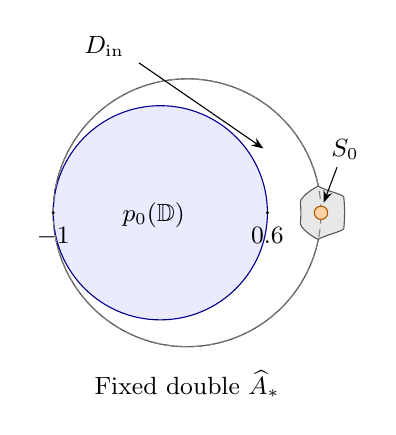
\begin{tikzpicture}[x=1.7cm,y=1.7cm,font=\small]
 \filldraw[fill=gray!18,draw=black!65]
  (11.4592:1) arc[start angle=11.4592,end angle=348.5408,radius=1]
  .. controls (1.045,-0.16) and (1.163,-0.14) .. (354.2704:1.1764706)
  arc[start angle=-5.7296,end angle=5.7296,radius=1.1764706]
  .. controls (1.163,0.14) and (1.045,0.16) .. (11.4592:1) -- cycle;
 \filldraw[fill=white,draw=black!65]
  (11.4592:1) arc[start angle=11.4592,end angle=348.5408,radius=1]
  .. controls (0.958,-0.192) and (0.862,-0.132) .. (354.2704:0.85)
  arc[start angle=-5.7296,end angle=5.7296,radius=0.85]
  .. controls (0.862,0.132) and (0.958,0.192) .. (11.4592:1) -- cycle;
 \filldraw[fill=blue!8,draw=blue!55!black] (-0.2,0) circle[radius=0.8];
 \draw[densely dashed,black!50] (0,0) circle[radius=1];
 \filldraw[fill=orange!35,draw=orange!70!black] (1,0) circle[radius=0.05];
 \node at (-0.25,-0.02) {$p_0(\mathbb D)$};
 \fill (-1,0) circle[radius=0.012];
 \fill (0.6,0) circle[radius=0.012];
 \node[below] at (-1,-0.04) {$-1$};
 \node[below] at (0.6,-0.04) {$0.6$};
 \node at (-0.62,1.24) {$D_{\rm in}$};
 \draw[-{Stealth[length=1.5mm]},thin] (-0.36,1.12) -- (0.57,0.48);
 \node at (1.18,0.47) {$S_0$};
 \draw[-{Stealth[length=1.5mm]},thin] (1.12,0.34) -- (1.02,0.075);
 \node at (0,-1.28) {Fixed double $\widehat A_*$};
\end{tikzpicture}
\end{minipage}\hfill
\begin{minipage}[c]{0.50\textwidth}
\centering
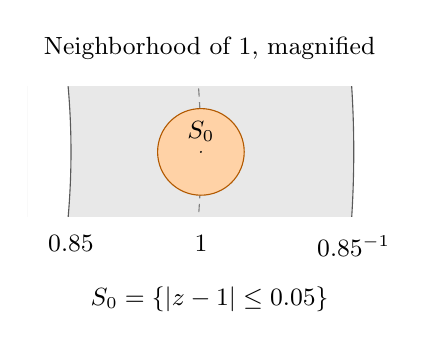
\begin{tikzpicture}[x=11cm,y=11cm,font=\small]
 \begin{scope}
  \clip (0.80,-0.075) rectangle (1.22,0.075);
  \fill[gray!18] (0,0) circle[radius=1.1764706];
  \fill[white] (0,0) circle[radius=0.85];
  \draw[black!65] (0,0) circle[radius=0.85];
  \draw[black!65] (0,0) circle[radius=1.1764706];
  \draw[densely dashed,black!50] (0,0) circle[radius=1];
  \filldraw[fill=orange!35,draw=orange!70!black] (1,0) circle[radius=0.05];
  \fill (1,0) circle[radius=0.0012];
 \end{scope}
 \node at (1.01,0.12) {Neighborhood of $1$, magnified};
 \node[below] at (0.85,-0.085) {$0.85$};
 \node[below] at (1,-0.085) {$1$};
 \node[below] at (1.17647,-0.085) {$0.85^{-1}$};
 \node at (1.01,-0.17) {$S_0=\{|z-1|\leq0.05\}$};
 \node at (1,0.024) {$S_0$};
\end{tikzpicture}
\end{minipage}
\caption{The fixed geometry used in the round-annulus factorization.
The blue disc $p_0(\mathbb D)$ lies in the incoming disc, and the orange
insertion disc lies strictly inside the gray doubled annulus.
The dashed curve is the unit-circle interface.  The transition curves
in the overview are schematic; the magnified panel uses the stated
radii on the central part of the dent.}
\label{fig:fixed-annulus}
\end{figure}

\emph{Factoring the shrinking annulus.}
The map $\gamma_t$ moves the fixed point $a$ to $r$.  We arrange the
remaining incoming boundary by writing
$s\operatorname{id}=\gamma_t\circ p_0\circ b_t$, namely by defining
\[
 b_t=p_0^{-1}\circ\gamma_t^{-1}\circ(s\operatorname{id}).
\]
After doubling, the factor $\gamma_t$ will cancel against its adjoint.
The insertion will then lie between the same fixed factors
$\underline C^*$ and $\underline C$, with only the contractions
$\underline b_t^*$ and $\underline b_t$ outside them.

The disc $\gamma_t^{-1}(s\mathbb D)$ has real diameter with endpoints
$-(s+t)/(1+st)>-1$ and $1/2$.  It lies strictly in $p_0(\mathbb D)$,
so $b_t$ is a strict Möbius disc embedding.  Its covered univalent lift
is a contraction, whereas the lift of $\gamma_t$ is unitary.  Choose
these lifts so that
\begin{equation}\label{eq:round-factorization}
 s^{L_0}=\underline\gamma_t\,
          \underline A_*\underline C\,\underline b_t
\end{equation}
is the standard round-annulus lift.  This is an equality in the covered
univalent semigroup, whose inclusion lifts to
$\widetilde{\operatorname{Ann}}_c$
\cite[Section~4.2]{HTVOA}: the Virasoro cocycle vanishes on the
univalent subalgebra, so this lift introduces no scalar ambiguity.
Any winding adjustment acts unitarily.

Consider the insertion coordinate
$p_t(\zeta)=\gamma_t^{-1}(r+q\zeta)$.  The identities
\[
 1-tr=\frac{1-t^2}{1+ta},\qquad
 \frac{q}{1-tr}=\frac{2(1-a^2)}{t+a}<0.000401,
\]
and
\[
 \gamma_t^{-1}(r+h)-a
   =\frac{(1-t^2)h}{(1-tr)(1-tr-th)}
\]
show, for $|h|\leq q$, that
\[
 |\gamma_t^{-1}(r+h)-a|
  \leq\frac{2(0.000401)}{1-0.000401}<0.000803.
\]
Consequently $p_t(\mathbb D)\subset\mathring S_0$ for every $t$.
The map has no pole there.  Also $s>t$, so the pole $1/t$ of
$\gamma_t^{-1}$ is outside the round annulus with outer radius $1/s$.
Since $\gamma_t$ commutes with reflection in the unit circle, we may
double \eqref{eq:round-factorization}, carrying along the insertion.
The unitary factors cancel, and gluing gives the exact operator identity
\begin{equation}\label{eq:round-doubled}
 A_{1/s,s,N}[(q^{L_0}v)(r)]
 =\underline b_{t,N}^{*}\underline C_N^{*}
    (\underline A_*^\dagger\underline A_*)_N[(p_t)_*v(0)]
    \underline C_N\underline b_{t,N}.
\end{equation}
\emph{The uniform bound.}
Lemma~\ref{lem:fixed-disc} bounds the middle factor by a fixed constant
times $\|v\|$.  Thus the right side has norm at most
$C_{\widehat A_*,S_0}\|\underline C_N\|^2\|v\|$.
In particular, no radius-dependent comparison scalar is introduced.

Finally,
\[
 \frac{1-s}{1-r}
 =5000\frac{1+ta}{1+t/2},
\]
which proves \eqref{eq:round-comparable}.
\end{proof}

\subsection{Transport forms and infinite insertion states}

Recall from \eqref{eq:creation} that, for a unitary module $M$, the creation and annihilation intertwiners are
\[
 \mathcal Y_M^+(a,z)v=e^{zL_{-1}}Y^M(v,-z)a,
 \qquad \mathcal Y_M^-=(\mathcal Y_M^+)^\dagger.
\]
Their types are respectively $\binom{M}{M\,V}$ and
$\binom{V}{\bar M\,M}$.  The charge transform \eqref{eq:theta-convention},
for a complex coordinate with a chosen logarithm, is
\[
 \theta_{\bar z}a
   =e^{\bar zL_1}e^{i\pi L_0}\bar z^{-2L_0}\bar a,
\]
using the conjugate logarithm at $\bar z$.
For unitary modules $M,N$, define the diagonal transport form by
\begin{equation}\label{eq:transport-form}
 \mathfrak t_z^{M,N}(a\otimes b,a'\otimes b')
 =\big\langle
 Y^N\big(\mathcal Y_M^-(\theta_{\bar z}a',
                         \bar z^{-1}-z)a,z\big)b,b'\big\rangle.
\end{equation}
We use this for $0<|z|<1$ and $|z|>|z|^{-1}-|z|$.
At positive real $z$ all positive-coordinate logarithms are real;
on a rotated diagonal the two insertion coordinates have the same
argument and the reflected logarithm is the conjugate one.  The form
is linear in its first entry.

Regularity gives absolute convergence of these matrix coefficients.
More precisely, the ordinary intertwiners between unitary modules have
Hilbert-space values at $0<|z|<1$, with branchwise norm holomorphy
\cite[Definition~2.8, Lemma~2.9 and Proposition~3.11]{TenerFusion}.
Creation satisfies the identity
\begin{equation}\label{eq:creation-transport}
 \mathfrak t_z^{M,V}(a\otimes b,a'\otimes b')
   =\langle\mathcal Y_M^+(a,z)b,
                  \mathcal Y_M^+(a',z)b'\rangle
\end{equation}
without assuming energy bounds, integration of $M$, or positivity of
general fusion forms \cite[Proposition~3.10]{TenerFusion}.

\begin{lemma}[Hilbert-state insertions]\label{lem:transport-cutoff}
Let $M,N$ be unitary modules, with $N$ already integrated.  For
homogeneous $a,a'\in M$ of weights $d,d'$, set
\[
 u_z=\mathcal Y_M^-(\theta_{\bar z}a',\bar z^{-1}-z)a,
 \qquad \delta=|z|^{-1}-|z|,\qquad q=2\delta.
\]
As $|z|$ tends to one on a fixed branch,
\begin{equation}\label{eq:annulus-hilbert-state}
 q^{-L_0}u_z\in\mathcal H_V,
 \qquad \|q^{-L_0}u_z\|\leq C_{a,a'}\delta^{-d-d'}.
\end{equation}
For a fixed dent with $z$ in its inner collar,
$\widehat A_N[u_z(z)]$ is well defined by norm limits of energy
truncations, belongs to $\pi_I^N(A_V(I))$, and has norm at most
$C\delta^{-d-d'}$.  On $\underline A_N^{-1}N$ in both variables it obeys
\begin{equation}\label{eq:transport-cutoff}
 \langle\widehat A_N[u_z(z)]\xi,\eta\rangle
 =\mathfrak t_z^{M,N}
   (a\otimes\underline A_N\xi,
    a'\otimes\underline A_N\eta).
\end{equation}
For the round annuli of Proposition~\ref{prop:round-annulus}, the same
bound holds with the cutoffs $s^{L_0}$ in both entries and $z=r$.
\end{lemma}

\begin{proof}
Expand $\theta_{\bar z}a'$ into finitely many vectors of weights
$d_j\leq d'$.  Their coefficients are bounded as $|z|$ tends to one.
By $L_0$-covariance, applying $q^{-L_0}$ to each annihilation value
produces the factor $q^{-d_j-d}$ and an annihilation value at modulus
$\delta/q=1/2$.  The latter is a Hilbert-space vector by
\cite[Proposition~3.11]{TenerFusion}; rotations preserve its norm.
This proves \eqref{eq:annulus-hilbert-state}.

Let $P_n$ be the vacuum energy cutoff.  Apply the uniform collar
version of \eqref{eq:fixed-disc-bound} to
$q^{-L_0}(P_n-P_m)u_z$.  It gives
\[
 \|\widehat A_N[(P_n u_z)(z)]
       -\widehat A_N[(P_m u_z)(z)]\|
 \leq C\|q^{-L_0}(P_n-P_m)u_z\|.
\]
Thus these operators converge in norm, with the asserted bound.
Locality and representation transfer persist under that norm limit.
For finite truncations, \eqref{eq:annulus-insertion} applies.
Absolute convergence of the transport iterate identifies its limiting
matrix coefficients on the exact dense preimages, proving
\eqref{eq:transport-cutoff}.  The identical argument using
\eqref{eq:uniform-round} and \eqref{eq:round-insertion} gives the
round-annulus assertion.
\end{proof}

\subsection{Charged modes and bounded boundary smears}

\begin{lemma}[Analytic tools for a dominated intertwiner]
\label{lem:charged-tools}
Let $M,N,K$ be grading-restricted unitary $V$-modules, with $N$ already
strongly integrable, and let $\Phi$ have type $\binom{K}{M\,N}$.
Fix a homogeneous $a\in M$ of weight $d$.  Suppose that, for all
finite-energy $b\in N$ and all diagonal positions sufficiently close
to the unit circle on the branches under consideration,
\begin{equation}\label{eq:transport-domination}
 \|\Phi(a,z)b\|^2
   \leq C_a\mathfrak t_z^{M,N}(a\otimes b,a\otimes b).
\end{equation}
Then $\Phi(a,z)$ has polynomial energy bounds, as do its levelwise
adjoint coefficients.  Its smooth smears and their formal adjoints
preserve the smooth domains continuously.

For every smooth test $f$ supported compactly in an interval $I$ with
a chosen argument, there is a localized radial annulus $\underline A$
with a dent over $\operatorname{supp}f$ such that
\begin{equation}\label{eq:charged-bounded-cutoff}
 T_f=\overline{\Phi(a,f)}\,\underline A_N
       :\mathcal H_N\longrightarrow\mathcal H_K
\end{equation}
is bounded and defined on all of $\mathcal H_N$.
Both $T_f$ and $T_f^*$ preserve smooth vectors in their respective
directions.  Moreover,
\[
 N\subset\operatorname{ran}\underline A_N,
 \qquad \underline A_N^{-1}N\text{ is dense in }\mathcal H_N.
\]
These conclusions apply to $\Phi=\mathcal Y_M^+$ and $N=V$ for every
already unitary $M$, before integrating $M$.
\end{lemma}

\begin{proof}
Lemma~\ref{lem:transport-cutoff} and
Proposition~\ref{prop:round-annulus} give
\begin{equation}\label{eq:charged-radial-estimate}
 \|\Phi(a,r)s^{L_0}b\|
      \leq C(1-r)^{-d}\|b\|,
 \qquad b\in N.
\end{equation}
Write the physical expansion as
$\Phi(a,z)=\sum_\mu\Phi(a)[\mu]z^{-\mu-d}$, so that a coefficient
maps energy $h$ to $h-\mu$.  For $b$ of energy $h$, project
\eqref{eq:charged-radial-estimate} to that output energy.  Fix
$0<\varepsilon_a\leq10^{-4}$ small enough that the transport domination
and the cutoff estimate hold whenever $1-\varepsilon_a\leq r<1$, and choose
\[
 1-r=\frac{\varepsilon_a}{1+h+|\mu|}.
\]
The corresponding $t$ lies in $[0,1)$.  By
\eqref{eq:round-comparable}, $s\geq1/2$ and
$1-s\leq(6667)10^{-4}/(1+h+|\mu|)$.
Since $-\log s\leq2(1-s)$, the factor $s^{-h}$ is uniformly bounded.
The factor $r^{\mu+d}$ is uniformly bounded as well, using $d\geq0$
and $r\geq1-10^{-4}$.  Hence
\begin{equation}\label{eq:charged-mode-estimate}
 \|\Phi(a)[\mu]b\|
     \leq C(1+h+|\mu|)^d\|b\|.
\end{equation}
Distinct input energies have distinct output energies for a fixed
coefficient.  Orthogonality therefore turns this into a polynomial
energy bound on $N$.  Taking adjoints between individual energy spaces
gives the same kind of bound for the adjoint coefficients.  Choose any
integer energy order at least $d$ when an integer order is desired.

On a fixed argument interval, define $\Phi(a,f)$ by smearing its physical
field $z^d\Phi(a,z)$ against $f(e^{i\vartheta})\,d\vartheta/(2\pi)$.
Other smooth weight factors can be absorbed into $f$.  Rapid decay of
Fourier coefficients, \eqref{eq:charged-mode-estimate}, and the energy
shifts show that this smear and its formal adjoint map smooth vectors
continuously to smooth vectors.  For clarity, a target Sobolev seminorm
of order $j$ is bounded by an input seminorm of a fixed higher order,
times a summable series of polynomially weighted Fourier coefficients.
This also shows that finite-energy truncations converge in the graph
norm of the smear.  The closures of the smears defined on finite-energy
and on smooth vectors consequently agree.

Choose $\underline A$ with $\rho<1$ on a neighborhood of
$\operatorname{supp}f$ and with $1-\rho$ compactly supported in $I$.
On the fixed dense subspace $\underline A_N^{-1}N$, consider
\[
 T(z)\xi=\Phi(a,z)\underline A_N\xi.
\]
The localized part of Lemma~\ref{lem:transport-cutoff}, together with
\eqref{eq:transport-domination}, gives a bounded extension satisfying
\begin{equation}\label{eq:charged-collar}
 \|T(z)\|\leq C(1-|z|)^{-d}
\end{equation}
throughout an inner collar over this neighborhood.  Its values on the
dense initial domain are Hilbert-valued holomorphic functions, by
\cite[Lemma~2.9 and Proposition~3.11]{TenerFusion}.
Local uniform boundedness therefore gives operator-norm holomorphy.

For neutral fields, annulus regularization and the Banach-valued
boundary argument appear in \cite[Proposition~8.4 and Lemma~8.5]{HTVOA}.
The charged collar estimate \eqref{eq:charged-collar} supplies the
hypothesis needed here. We spell out the boundary argument.
Put
\[
 F_f(t)=\int f(e^{i\vartheta})e^{id\vartheta}
                         T(te^{i\vartheta})\,\frac{d\vartheta}{2\pi}.
\]
All integrals here use the chosen argument and the compact support of
$f$.  Holomorphy gives $t\partial_tT=-i\partial_\vartheta T$.
After integrating by parts, every radial derivative of order $p$ of
$F_f$ is a finite sum of integrals of $T$ against derivatives of the
fixed smooth test, multiplied by bounded powers of $t^{-1}$.
Thus
\[
 \|F_f^{(p)}(t)\|\leq C_{f,p}(1-t)^{-d}.
\]
Choose an integer $p>d$.  Taylor's integral formula from a fixed
$t_0<1$ expresses $F_f(t)$ as a polynomial plus the integral of
$(t-u)^{p-1}F_f^{(p)}(u)/(p-1)!$.
The norm of the latter integrand is bounded, uniformly for $u\leq t$,
by a constant times $(1-u)^{p-1-d}$, which is integrable at one.
Dominated convergence proves that $F_f(t)$ has an operator-norm limit
$T_f$ as $t$ tends to one.

On $\underline A_N^{-1}N$, the mode expansion and its polynomial bounds
identify this limit with $\Phi(a,f)\underline A_N$.
For arbitrary $\xi\in\mathcal H_N$, approximate $\xi$ by
$\xi_j\in\underline A_N^{-1}N$.  Then
$\underline A_N\xi_j\to\underline A_N\xi$ and
$T_f\xi_j\to T_f\xi$.  Closedness of the smeared field proves
\eqref{eq:charged-bounded-cutoff} on all of $\mathcal H_N$.
Lemma~\ref{lem:annulus-range} supplies the asserted range and density.

The product in \eqref{eq:charged-bounded-cutoff} preserves smooth
vectors, since both its factors do.  If $\Phi(a,f)^\dagger$ denotes
the formal adjoint smear, then every smooth target vector $\eta$
belongs to the adjoint domain of $\overline{\Phi(a,f)}$, and
\[
 T_f^*\eta=\underline A_N^*\Phi(a,f)^\dagger\eta.
\]
Indeed this equality follows by pairing with the dense finite-energy
core and using the adjoint coefficient bounds.  The right side is
smooth: the formal adjoint smear preserves smooth vectors and the
fixed annulus adjoint preserves every Sobolev space.  This proves the
remaining domain assertion.  Finally,
\eqref{eq:creation-transport} supplies
\eqref{eq:transport-domination} with constant one for creation, with
the vacuum as its integrated source.
\end{proof}

\section{Integrating the unitary modules}
\label{sec:integration}

We now construct the local algebra actions on a unitary module.
The input is the bounded regularization of a charged field from
Lemma~\ref{lem:charged-tools}.  We first show that this regularization
intertwines the observables in a disjoint interval as closed operators.
Creation fields will then identify the observable algebra on the module
with the vacuum algebra.  Only the already given positive form on the
module is used in this construction.

For unitary modules $N,K$ and an interval $J$, define the diagonal
observable algebra
\begin{equation}
 \mathcal B_{N,K}(J)=W^*\!\left\{
 \overline{Y^N(v,g)}\oplus\overline{Y^K(v,g)}:
 v\in V\text{ homogeneous},\ 
 g\in C_c^\infty(J)\right\}.
 \label{eq:diagonal-observable-algebra}
\end{equation}
As for $A_V$, an unbounded generator means its closed graph data,
or equivalently its bounded transform and polar data.  If
$T:\mathcal H_N\to\mathcal H_K$ is a closed densely defined operator,
its closed lower-corner operator on $\mathcal H_N\oplus\mathcal H_K$ is
\[
 \widetilde T=\begin{pmatrix}0&0\\T&0\end{pmatrix},
 \qquad\Dom\widetilde T=\Dom T\oplus\mathcal H_K.
\]
We say that $T$ \emph{strongly intertwines the observables in $J$}
when $\widetilde T$ is affiliated with $\mathcal B_{N,K}(J)'$.

\begin{proposition}[Strong intertwining from annulus regularization]
\label{prop:strong-intertwining}
Let $V$ be simple, unitary and strongly rational, and let $M,N,K$ be
grading-restricted unitary $V$-modules, with $N$ strongly integrable.
Let $\Phi$ be an intertwining operator of type $\binom{K}{M\,N}$,
and let $a\in M$ be homogeneous.  Assume that $\Phi(a,z)$ satisfies
the transport domination hypothesis of Lemma~\ref{lem:charged-tools}.
Smear $\Phi(a,z)$ against a smooth test $f$ supported in an interval $I$, with
a fixed argument branch.  If $J$ is disjoint from $I$, then the closed
smeared operator $\overline{\Phi(a,f)}$ strongly intertwines the
diagonal smeared observables of $N$ and $K$ supported in $J$.
This holds for every homogeneous observable in $V$ and for every such
choice of tests and argument branches.
\end{proposition}

\begin{proof}
Write $\mathcal D_N=\mathcal H_N^\infty$ and
$\mathcal D_K=\mathcal H_K^\infty$.
The polynomial mode estimates imply that smeared fields and their formal
adjoints map the corresponding smooth spaces continuously to smooth
spaces.  Spectral truncations converge in all the smooth seminorms.
Consequently a smear has the same closure whether it is initially
defined on finite-energy vectors or on smooth vectors.  These facts
apply both to the observables and, by Lemma~\ref{lem:charged-tools},
to the charged field.

Choose the localized annulus $\underline A$ in that lemma with its dent
containing $\operatorname{supp}f$ and localized in $I$.
Its action $\underline A_N$ is a
bounded injective operator with dense range, and
\begin{equation}
 T_f=\overline{\Phi(a,f)}\underline A_N
 \label{eq:bounded-charge-regularization}
\end{equation}
is bounded on all of $\mathcal H_N$.  Both $T_f$ and $T_f^*$ preserve
the respective smooth spaces.  On $\mathcal D_K$ the adjoint is
$\underline A_N^*\Phi(a,f)^\dagger$, where the dagger denotes the formal smeared
adjoint.  These are assertions about the full bounded regularization,
not merely about its restriction to finite energies.

For homogeneous $v\in V$ and a smooth $g$ supported in $J$, put
\[
 S_N=\overline{Y^N(v,g)},\qquad
 S_K=\overline{Y^K(v,g)}.
\]
On the smooth spaces, the intertwining-operator Jacobi identity gives
\[
 Y^K(v,g)\Phi(a,f)=\Phi(a,f)Y^N(v,g).
\]
To pass from the formal identity to this equality, multiply the two
field orderings by a sufficiently high integral power of the coordinate
difference.  Polynomial energy bounds make the resulting series
smooth-domain distributions.  Since the two test supports are
disjoint, one can divide the product test by that power.  The same
argument applies to the adjoint relation, whose observable test has
the same support.  This is the weak intertwining property in
\cite[Theorem~3.5]{GuiUnbounded}.

The operator $\underline A_N$ and its adjoint commute strongly with these
observables: $\underline A_N$ is localized in $I$, whereas $N$ is already
integrated and the observables are localized in $J$.
Combining this with the weak identities gives
\begin{equation}
 S_KT_f\xi=T_fS_N\xi\quad(\xi\in\mathcal D_N),
 \qquad
 S_NT_f^*\eta=T_f^*S_K\eta\quad(\eta\in\mathcal D_K).
 \label{eq:bounded-charge-core-commutation}
\end{equation}
For the second equality one can pair the first weak intertwining
identity for the \emph{formal adjoint observable}.  More explicitly,
let $S_N^\dagger$ and $S_K^\dagger$ denote its actions on the smooth
spaces.  The invariant adjoint formula expresses it as a finite sum
of smears of PCT-transformed states and their $L_1$-descendants, with
tests still supported in $J$.  Thus the first equality also gives
$T_fS_N^\dagger=S_K^\dagger T_f$ on $\mathcal D_N$.
For $\xi\in\mathcal D_N$ and $\eta\in\mathcal D_K$, using our
linear-first inner product convention, we obtain
\[
\begin{aligned}
 \langle S_NT_f^*\eta,\xi\rangle
 &=\langle T_f^*\eta,S_N^\dagger\xi\rangle
  =\langle\eta,T_fS_N^\dagger\xi\rangle\\
 &=\langle\eta,S_K^\dagger T_f\xi\rangle
  =\langle S_K\eta,T_f\xi\rangle
  =\langle T_f^*S_K\eta,\xi\rangle.
\end{aligned}
\]
All vectors in these pairings are smooth.  This proves the second
equality in \eqref{eq:bounded-charge-core-commutation} without
identifying a formal-adjoint closure with the full Hilbert-space
adjoint.

We spell out the passage to closed operators.  On
$\mathcal H_N\oplus\mathcal H_K$, let
\[
 D=S_N\oplus S_K,\qquad
 Q_f=\begin{pmatrix}0&0\\T_f&0\end{pmatrix}.
\]
Approximation in the graph norms, using the smooth cores, shows that
both $Q_f$ and $Q_f^*$ preserve $\operatorname{Dom}D$ and commute with
$D$ there.  Hence $Q_f\oplus Q_f$ and its adjoint preserve the closed
graph of $D$.  They therefore commute with its orthogonal projection.
The matrix entries of this graph projection determine the usual
bounded transform and polar data of $D$.  Thus $Q_f$ commutes with the
von Neumann algebra generated by $D$.

As $v$ and $g$ vary, the preceding argument proves
$Q_f\in\mathcal B_{N,K}(J)'$.

It remains to remove the annulus.  The first-summand compression of
$\mathcal B_{N,K}(J)$ is $\pi_J^N(A_V(J))$: its normal range is
generated by the module smears, which are the images of the vacuum
generators under strong integration.  Since $\underline A_N$ is
localized in $I$, both $\operatorname{diag}(\underline A_N,1)$ and
its adjoint commute with $\mathcal B_{N,K}(J)$.  The closed inverse
$\underline A_N^{-1}$ is densely defined on
$\operatorname{ran}\underline A_N$, and inversion preserves the
resulting affiliation with the commutant.  Therefore
\[
 Q_f\begin{pmatrix}\underline A_N^{-1}&0\\0&1\end{pmatrix}
\]
is densely defined, and its domain and action commute with every
unitary in $\mathcal B_{N,K}(J)$.  It is closable: by
\eqref{eq:bounded-charge-regularization} it is a restriction of the
closed operator with lower corner $\overline{\Phi(a,f)}$ and all other
corners zero.  Its domain contains the finite-energy core in the first
summand, since $N\subset\operatorname{ran}\underline A_N$ by
Lemma~\ref{lem:annulus-range}.  Its closure is consequently exactly
that closed lower-corner operator.  This proves its affiliation with
$\mathcal B_{N,K}(J)'$.

This affiliation is the strong intertwining assertion, including the
diagram convention used in \cite[Section~3.3]{GuiUnbounded}.
Explicitly, on two copies of $\mathcal H_N\oplus\mathcal H_K$, repeat
the charged corner diagonally and place a diagonal observable in a
matrix corner between the copies.  The latter is affiliated with
$M_2(\mathcal B_{N,K}(J))$, and the repeated charged corner with its
commutant.  Hence the diagram commutes strongly.  All operations above
are valid for each fixed branch on $I$.
\end{proof}

We next use creation fields to show that the vacuum compression of a
diagonal observable algebra loses no information.

\begin{lemma}[Totality of local creation ranges]
\label{lem:creation-totality}
Let $V$ be simple, unitary and strongly rational, let $M$ be a
grading-restricted unitary $V$-module, and let $I$ be a nonempty
interval.  For every homogeneous $a\in M$ and
$f\in C_c^\infty(I)$, form the bounded creation regularization
\[
 T_{a,f}=\overline{\mathcal Y_M^+(a,f)}\underline A_V
\]
of Lemma~\ref{lem:charged-tools}; the localized annulus may depend on
the test.  The closed linear span of their ranges is $\mathcal H_M$.
\end{lemma}

\begin{proof}
The transport domination needed here holds with equality for creation
and vacuum source.  It uses the given form on $M$, and assumes neither
integration of $M$ nor positivity of a general fusion product.
Since $\Omega\in\operatorname{ran}\underline A_V$, each range contains
$\mathcal Y_M^+(a,f)\Omega$.

Suppose $\eta\in\mathcal H_M$ is orthogonal to all these vectors.
For each homogeneous $a$, consider
\[
 F_a(z)=\langle e^{zL_{-1}}a,\eta\rangle,
 \qquad |z|<1.
\]
Creation gives
$\mathcal Y_M^+(a,z)\Omega=e^{zL_{-1}}a$.
The charged energy estimate bounds the Taylor coefficients of $F_a$
by a polynomial in their index.  Its boundary value is therefore a
distribution with only nonnegative Fourier frequencies.  Orthogonality
to all the creation smears says that this distribution vanishes on
$I$.  The smooth weight or branch factor in the smearing convention
can be absorbed into the test on this interval.

For completeness, such a one-sided distribution is zero if it vanishes
on a nonempty arc.  Convolve it with smooth approximate identities
supported in increasingly small arcs.  Each convolution still has
only nonnegative frequencies and vanishes on a smaller nonempty arc.
It is the smooth boundary value of a holomorphic function in the disc.
The Schwarz reflection principle across an arc on which that function
is zero, followed by analytic uniqueness, shows that the convolution
is identically zero.  Passing to the distributional limit proves the
claim.  Thus $F_a=0$, and its constant coefficient gives
$\langle a,\eta\rangle=0$.  Homogeneous vectors span $M$, which is
dense in $\mathcal H_M$; hence $\eta=0$.
\end{proof}

Local-intertwiner criteria for module integration are given in
\cite[Proposition~4.7]{GuiUnitaryII} and
\cite[Lemma~4.27]{GuiExtensions}. The following diagonal-algebra proof
uses the bounded creation operators and their total ranges to establish
the representations together with equality of the full closed graphs.

\begin{theorem}[Strong integration of every unitary module]
\label{thm:integration}
Let $V$ be simple, unitary and strongly rational.  Every
grading-restricted unitary $V$-module $M$ has a unique compatible
family of normal representations
\[
 \pi_J^M:A_V(J)\longrightarrow B(\mathcal H_M)
\]
such that, for every homogeneous $v\in V$ and
$g\in C_c^\infty(J)$,
\begin{equation}
 \pi_J^M\!\left(\overline{Y^V(v,g)}\right)
       =\overline{Y^M(v,g)}.
 \label{eq:exact-cwx-smear}
\end{equation}
Equality here includes the domains of the closed affiliated operators.
The canonical Virasoro action of this net representation is the
integrated module Virasoro action; in particular its rotations are
$e^{itL_0}$ with the module's conformal-energy normalization.
\end{theorem}

\begin{proof}
Module energy bounds follow from Theorem~\ref{thm:energy}, and the
vacuum net exists by Corollary~\ref{cor:locality}.
Fix $J$ and form $\mathcal B(J)=\mathcal B_{V,M}(J)$ as in
\eqref{eq:diagonal-observable-algebra}, including every homogeneous
observable.  Its two Hilbert summands reduce all its generators.
Vacuum restriction is therefore a normal unital homomorphism
\[
 r_0:\mathcal B(J)\longrightarrow A_V(J).
\]
It is onto.  Indeed, compression of the graph data of a direct sum
gives the graph data of its first summand, and these compressed data
generate $A_V(J)$.  The range of a normal homomorphism of von Neumann
algebras is a von Neumann algebra, so it contains that generated
algebra and is equal to it.

The kernel of $r_0$ is $\mathcal B(J)q$ for a central projection $q$.
Choose any interval $I$ disjoint from $J$.  Apply
Proposition~\ref{prop:strong-intertwining} to creation, whose source
is the integrated vacuum.  Its bounded regularizations commute, as
lower corners, with $\mathcal B(J)$.  Since $q$ annihilates the vacuum
summand, its restriction $q_M$ to the other summand satisfies
\[
 q_MT_{a,f}=T_{a,f}q_V=0.
\]
Lemma~\ref{lem:creation-totality} gives $q_M=0$, hence $q=0$.
Thus $r_0$ is a normal isomorphism.  Its inverse is normal as well:
an order isomorphism preserves suprema of bounded increasing positive
nets.  If $r_M$ denotes restriction to the module summand, define
\[
 \pi_J^M=r_Mr_0^{-1}.
\]
For $J_1\subset J_2$ the diagonal algebras are nested, and both
compression maps respect the inclusions.  It follows that
$\pi_{J_2}^M|_{A_V(J_1)}=\pi_{J_1}^M$.

We verify the exact closed-operator identity.
Let $S_V=\overline{Y^V(v,g)}$ and
$S_M=\overline{Y^M(v,g)}$.
The graph projection of $S_V\oplus S_M$ has its matrix entries in
$\mathcal B(J)$.  Compressing its entries to the two summands yields
the graph projections of $S_V$ and $S_M$, respectively.
Consequently the matrix amplification of $\pi_J^M$ sends the entire
graph projection of $S_V$ to that of $S_M$.  This is precisely the
normal image of an affiliated closed operator, and proves
\eqref{eq:exact-cwx-smear}.  In particular the argument identifies
closed graphs, rather than merely operators on a dense common domain.

The graph data of the vacuum smears generate each $A_V(J)$, so the
same identity also proves uniqueness.  With the module energy bounds,
it is the defining property of strong integrability and of the CWX
action; see \cite[Definition~4.22]{GuiExtensions}.
Applying the identity to the conformal vector identifies all localized
stress-energy fields.  Their canonical centrally extended Virasoro
actions agree by \cite[Proposition~3.10]{GuiUnbounded}, equivalently
\cite[Remark~4.23]{GuiExtensions}.  This gives exactly $e^{itL_0}$
for rotations, not an arbitrarily shifted positive-energy generator.
The normalization is important when using $r^{L_0}$ in annulus
factorizations.
\end{proof}

The construction respects finite orthogonal sums.  This follows either
from the closed-smear identity and uniqueness, or directly from the
diagonal construction.  Thus the theorem applies to all objects of
the grading-restricted unitary category, including finite sums of the
vacuum.  It makes no assertion yet that every simple algebraic module
admits such a positive form.  We establish that remaining assertion
after proving positivity of transport for pairs of unitary modules.

\section{Positive forms on fusion products}
\label{sec:fusion}

We now use the normal representations constructed in
Theorem~\ref{thm:integration} to transfer a vacuum Gram matrix to an
arbitrary unitary module.  The algebraic fusion product need not yet be
unitary.  We first construct a nondegenerate invariant sesquilinear form
on that product, and then prove its positivity separately on every
conformal-energy space.

For unitary modules $M,N$, extend the diagonal transport form
\eqref{eq:transport-form} to positive real insertion points by setting
\begin{equation}
\begin{split}
 \mathfrak t^{M,N}_{z,w}(a\otimes b,a'\otimes b')
 =\big\langle
 Y^N\big(\mathcal Y_M^-(\theta_w a',w^{-1}-z)a,z\big)b,b'
 \big\rangle_N,
\end{split}
\label{eq:two-point-transport}
\end{equation}
where $a,a'\in M$, $b,b'\in N$, and
\begin{equation}
 0<z,w<1,\qquad w^{-1}>z>w^{-1}-z>0.
 \label{eq:positive-transport-region}
\end{equation}
As usual, insertion of a vector in the grade completion means the
absolutely convergent sum over its homogeneous components.  Thus
$\mathfrak t^{M,N}_{r,r}=\mathfrak t^{M,N}_r$ in the notation of
Section~\ref{sec:annuli}.

\begin{theorem}[Positive fusion forms]
\label{thm:positive-fusion}
Let $V$ be a simple unitary strongly rational VOA.  For any unitary
grading-restricted finite-length $V$-modules $M,N$, let
$X=M\boxtimes N$ and let $\mathcal Y_X$ be its universal intertwining
operator.  There is a positive-definite invariant Hermitian form $h_X$
on $X$ such that
\begin{equation}
 \mathfrak t^{M,N}_{z,w}(a\otimes b,a'\otimes b')
 =\sum_\lambda h_X\big(
 \Pi_\lambda\mathcal Y_X(a,z)b,
 \Pi_\lambda\mathcal Y_X(a',w)b'\big)
 \label{eq:positive-fusion-identity}
\end{equation}
for all the vectors and coordinates in
\eqref{eq:two-point-transport}--\eqref{eq:positive-transport-region}.
The sum converges absolutely.  This is the canonical positive
normalization of the fusion form.
\end{theorem}

We prove the theorem in the next three subsections and check its
normalization in the fourth.

\subsection{A positive matrix in the local algebra}

We begin with positivity of the diagonal form.  Fix an interval $I$ near
$1\in S^1$, a localized dented annulus $\underline A$ as in
Section~\ref{sec:annuli}, and its double
$\widehat A=\underline A^\dagger\underline A$.  Choose a real $r<1$
sufficiently close to $1$ in its inner collar.  This choice works for
every finite list of charge vectors; constants in estimates may depend
on that list.  Write $\delta=r^{-1}-r$ and $q=2\delta$.

For $a_1,\ldots,a_m\in M$, set
\[
 u_{ij}=\mathcal Y_M^-(\theta_r a_i,\delta)a_j
 \quad\text{in the grade completion of }V.
\]
By linearity and \eqref{eq:annulus-hilbert-state},
$q^{-L_0}u_{ij}\in\mathcal H_V$.  The fixed-disc estimate
\eqref{eq:fixed-disc-bound} therefore defines bounded operators
\begin{equation}
 K_{ij}=\widehat A_V[u_{ij}(r)]\in A_V(I)
 \label{eq:local-transport-matrix}
\end{equation}
as operator-norm limits of the insertions of the finite level
truncations of $u_{ij}$.  In particular these limits remain in the
same local von Neumann algebra.

The vacuum transport identity for creation, namely
Proposition~3.10 of~\cite{TenerFusion}, and the insertion identity
\eqref{eq:annulus-insertion} give
\begin{equation}
 K_{ij}=T_i(r)^*T_j(r),\qquad
 T_j(r)=\mathcal Y_M^+(a_j,r)\underline A_V.
 \label{eq:transport-gram}
\end{equation}
Here the creation operators with the displayed cutoff are bounded by
Lemma~\ref{lem:charged-tools}.  The equality is first an equality of
matrix elements on $\underline A_V^{-1}V$, which is dense by
Lemma~\ref{lem:annulus-range}; boundedness extends it to the Hilbert
space.  Thus $(K_{ij})_{i,j=1}^m$ is a positive element of
$M_m(A_V(I))$.

By Theorem~\ref{thm:integration}, $N$ has a normal local representation
$\pi_I^N$.  Applying its matrix amplification preserves this
positivity.  For arbitrary $b_1,\ldots,b_m\in N$, choose exact
preimages $\xi_i$ under $\underline A_N$ as follows.  If the
complementary annulus of Lemma~\ref{lem:annulus-range} satisfies
$\underline A_N\underline B_N=s^{L_0}$, put
\[
 \xi_i=\underline B_Ns^{-L_0}b_i.
\]
The inverse power acts on a finite-energy vector, so this expression
is defined and $\underline A_N\xi_i=b_i$.  The norm-convergent
insertion identity, followed by absolute convergence of the
transport series, now gives
\begin{equation}
 \sum_{i,j=1}^m
 \mathfrak t^{M,N}_{r,r}(a_j\otimes b_j,a_i\otimes b_i)
 =\sum_{i,j=1}^m
 \langle\pi_I^N(K_{ij})\xi_j,\xi_i\rangle_N
 \geq0.
 \label{eq:transport-positive}
\end{equation}
Only the creation case was used to obtain the vacuum matrix.  General
fusion positivity has not entered this argument.

\subsection{The invariant form on the algebraic fusion object}

Assume first that $M,N$ are simple.  Associativity in the
positive-real region produces an intertwining operator $B$ of type
$\binom{N}{\bar M\ X}$ such that
\begin{equation}
 Y^N\big(\mathcal Y_M^-(c,w^{-1}-z)a,z\big)b
 =B(c,w^{-1})\mathcal Y_X(a,z)b
 \label{eq:fused-evaluation}
\end{equation}
in convergent matrix elements, for $c\in\bar M$, $a\in M$ and
$b\in N$.  Its morphism is the associator
followed by the annihilation morphism
$\bar M\boxtimes M\longrightarrow V$ and the left unit action on
$N$.  The annihilation is nonzero: its adjoint is creation, which
sends $a\otimes\Omega$ to $e^{zL_{-1}}a$.  Since $M$ is simple,
unitarity identifies $\bar M$ with $M^\vee$, and the annihilation
morphism is a nonzero multiple of rigid evaluation.  We also write
$B$ for its corresponding morphism.  Consequently
rigidity gives an isomorphism
\begin{equation}
 \operatorname{Hom}_V(E,X)\longrightarrow
 \operatorname{Hom}_V(\bar M\boxtimes E,N),
 \qquad f\longmapsto B(1_{\bar M}\boxtimes f)
 \label{eq:rigid-transport-adjunction}
\end{equation}
for every grading-restricted finite-length module $E$.

To turn \eqref{eq:fused-evaluation} into a form, recall the Hermitian
duality from Section~\ref{sec:preliminaries}, which does not require
positive forms.  For a module $E$, its conjugate
$\bar E$ has mode action
\[
 v_{(n)}^{\bar E}\bar x
   =\overline{(\Theta v)_{(n)}^E x}.
\]
Its Hermitian dual is $E^{\mathrm h}=(\bar E)^\vee$, with pairing
\begin{equation}
 [x,\lambda]_E=\overline{\lambda(\bar x)}.
 \label{eq:hermitian-dual-pairing}
\end{equation}
The pairing is linear in $x$ and conjugate-linear in $\lambda$.
Restricted contragredience gives its invariant adjoint relation.
The given inner product of $N$ is represented by a linear module
isomorphism $H_N:N\longrightarrow N^{\mathrm h}$.

Conjugate $B$ and apply the FHL contragredient transformation
\cite[Section~5.5]{FHL}, in the explicit algebraic form
\cite[Equation~(3.87), Proposition~3.46]{HLZII}, taking the integer
branch index in that formula to be $-1$.  Thus we use
\[
 e^{wL_1}e^{-i\pi L_0}w^{-2L_0}
\]
on the conjugated charge, and precompose the second input with
$H_N$.  This gives an intertwining
operator $B^\sharp$ of type $\binom{X^{\mathrm h}}{M\ N}$ with
\begin{equation}
 [x,B^\sharp(a,w)b]_X
   =\langle B(\theta_w a,w^{-1})x,b\rangle_N
 \qquad(x\in X,\ a\in M,\ b\in N, w>0).
 \label{eq:hermitian-dual-adjoint}
\end{equation}
The minus phase before conjugation gives the plus phase in
$\theta_w$.  All module weights are real, so these transformations
also preserve the prescribed positive-real branches.
Universality of $\mathcal Y_X$ gives a module map
$H:X\longrightarrow X^{\mathrm h}$ such that
$B^\sharp=H\mathcal Y_X$.

The map $H$ is surjective.  To see the role of rigidity, suppose that
the quotient map $q:X^{\mathrm h}\longrightarrow C=\operatorname{coker}H$
has nonzero target.  Hermitian duality identifies
$(X^{\mathrm h})^{\mathrm h}$ with $X$, so dualizing $q$ gives a
nonzero injection
\[
 f=q^{\mathrm h}:E=C^{\mathrm h}\longrightarrow X,
 \qquad f^{\mathrm h}H=qH=0.
\]
Pairing \eqref{eq:hermitian-dual-adjoint} with $f(E)$ would imply
$B(1_{\bar M}\boxtimes f)=0$: the charge transformation $\theta_w$
is invertible, and the pairing with $N$ is nondegenerate.  This
contradicts \eqref{eq:rigid-transport-adjunction}.  Hermitian duality
preserves finite length, so the surjective map $H$ is an isomorphism.

We have therefore constructed the nondegenerate invariant
sesquilinear form
\begin{equation}
 h_X(x,y)=[x,Hy]_X.
 \label{eq:algebraic-fusion-form}
\end{equation}
It pairs distinct energy spaces to zero.  At this stage neither
Hermitian symmetry nor positivity has been assumed.  Combining
\eqref{eq:fused-evaluation} and
\eqref{eq:hermitian-dual-adjoint} proves
\eqref{eq:positive-fusion-identity} for this form.  Absolute
convergence is the ordinary convergence of the product of $B$ and
$\mathcal Y_X$, applied to the restricted-dual functional supplied
by a finite-energy vector of $N$.

\subsection{Extracting positivity at one energy}

The positivity in \eqref{eq:transport-positive} concerns a sum over
all output energies.  The following lemma separates those energies
without first constructing a norm on $X$.

\begin{lemma}[Positive polynomial moments]
\label{lem:positive-moments}
Let $\Lambda\subset\mathbb R$ be countable and bounded below.
Suppose complex numbers $c_\lambda$ satisfy
\[
 \sum_{\lambda\in\Lambda}e^{\epsilon\lambda}|c_\lambda|<\infty
 \quad\text{for some }\epsilon>0.
\]
If $\sum_\lambda |p(\lambda)|^2c_\lambda$ is real and nonnegative
for every complex polynomial $p$, then every $c_\lambda$ is real
and nonnegative.
\end{lemma}

\begin{proof}
Set $\mu=\sum_\lambda c_\lambda\delta_\lambda$.  Polynomials are
dense in $L^2(|\mu|)$.  To see this, let $g$ be orthogonal to them.
Cauchy--Schwarz and the exponential moment show that the finite
complex measure $g\,|\mu|$ has an exponential moment of smaller
positive order.  Its bilateral Laplace transform is holomorphic in
a strip containing the imaginary axis.  Orthogonality makes every
derivative at zero vanish, so the identity theorem makes the
transform zero on this strip.  Uniqueness of the Fourier transform
of a finite measure then gives $g\,|\mu|=0$.  For completeness, this
last uniqueness follows by convolving the measure with Gaussian
approximate identities: every convolution has zero Fourier
transform and is zero, and the convolutions converge weakly to the
measure.

For a fixed $\lambda$, approximate the indicator of its atom by
polynomials $p_n$ in $L^2(|\mu|)$.  Then
$|p_n|^2$ converges to that indicator in $L^1(|\mu|)$, because
\[
 \big\||p_n|^2-|p_m|^2\big\|_{L^1(|\mu|)}
 \leq\|p_n-p_m\|_{L^2(|\mu|)}
       \big(\|p_n\|_{L^2(|\mu|)}+\|p_m\|_{L^2(|\mu|)}\big).
\]
Thus the nonnegative integrals $\int |p_n|^2\,d\mu$ tend to
$c_\lambda$.
\end{proof}

Fix the radius $r$ used in \eqref{eq:transport-positive}.  Consider
a finite sum in the grade completion,
\[
 x=\sum_i\mathcal Y_X(a_i,r)b_i,
 \qquad x_\lambda=\Pi_\lambda x,
 \qquad c_\lambda=h_X(x_\lambda,x_\lambda).
\]
After decomposing the inputs, we may take all $a_i,b_i$
homogeneous.  The numbers $c_\lambda$ have an exponential moment
in absolute value.  Indeed, choose $z>r$ sufficiently close to $r$
that $z<r^{-1}$.  In the absolutely convergent product with the
outer insertion fixed at $r^{-1}$, replacing the inner radius $r$
by $z$ multiplies its component of weight $\lambda$ by
\[
 (z/r)^{\lambda-\operatorname{wt}(a_i)-\operatorname{wt}(b_i)}.
\]
Absolute product convergence for each of the finitely many pairs
of inputs gives
$\sum_\lambda e^{\epsilon\lambda}|c_\lambda|<\infty$ for a
common $\epsilon>0$.  This uses only the sesquilinear form
\eqref{eq:algebraic-fusion-form} and algebraic convergence.

The space of such finite sums $x$ is stable under $L_0$, since
\begin{equation}
 L_0\mathcal Y_X(a,r)b
 =\mathcal Y_X(L_0a,r)b+\mathcal Y_X(a,r)L_0b
   +r\mathcal Y_X(L_{-1}a,r)b.
 \label{eq:fixed-radius-L0}
\end{equation}
The radius $r$ stays fixed in this step.  Each polynomial in $L_0$
introduces only finitely many further charge and source vectors, and
the fixed-disc construction of \eqref{eq:transport-positive} applies
at this same $r$ to every such finite list.  Its constants may change;
its positivity conclusion does not.
Apply \eqref{eq:transport-positive} to $p(L_0)x$.  Grade
orthogonality gives
\[
 \sum_\lambda |p(\lambda)|^2h_X(x_\lambda,x_\lambda)\geq0.
\]
Lemma~\ref{lem:positive-moments} proves
$h_X(x_\lambda,x_\lambda)\geq0$ at each energy.

These $x_\lambda$ run through the whole space $X_\lambda$.  In
fact the span of all coefficients of $\mathcal Y_X(a,z)b$ is a
graded submodule by the intertwiner commutator formula.  The
quotient map by that submodule has zero postcomposition with the
universal intertwiner, and is therefore zero.  For homogeneous
inputs each projection at the fixed nonzero radius $r$ is a
nonzero scalar multiple of its coefficient.  This proves the
asserted spanning at each energy.

It follows by polarization that $h_X$ is Hermitian and positive
semidefinite on every energy space, and hence on $X$.  A
zero-norm vector for a positive semidefinite Hermitian form belongs
to its radical.  Nondegeneracy of \eqref{eq:algebraic-fusion-form}
therefore makes $h_X$ positive definite.  In particular, $X$ is now
a unitary module.  Finite orthogonal decompositions of $M,N$
extend the construction to arbitrary unitary finite-length
modules: creation, annihilation and the transport identity split
in exactly these orthogonal blocks.

\subsection{Canonical normalization and general charged fields}

With $h_X$ now positive, \eqref{eq:hermitian-dual-adjoint} says
that $B$ is the adjoint of $\mathcal Y_X$ in Tener's convention.
Thus \eqref{eq:fused-evaluation} is the exact normalized
fusion identity for that convention.

We check the normalization, since fractional charge weights make
the adjoint phase significant.  Put, for $x>0$,
\[
 U_\pm(x)=e^{xL_1}e^{\pm i\pi L_0}x^{-2L_0}.
\]
Gui's contragredient convention is
$U_+(x)$ in~\cite[Equations~(8.3)--(8.5)]{GuiPositivity}; solving
for the adjoint uses
$U_-(x)=U_+(x^{-1})^{-1}$.  On a simple charge module of lowest
weight $h$, $U_-=e^{-2\pi i h}U_+$.  With inner products linear in
the first variable, this means that Gui's adjoint, after the
unitary identification of the conjugate charge with the
contragredient charge, is $e^{2\pi i h}$ times Tener's adjoint.
Gui's annihilation operator has the same factor relative to
$\mathcal Y_M^-$: its vacuum coefficient on a top vector $a$ is
$e^{i\pi h}x^{-2h}\|a\|^2$, whereas the coefficient for
$\mathcal Y_M^-$ is $e^{-i\pi h}x^{-2h}\|a\|^2$.

The two factors cancel in the fusion identity
\cite[Equation~(8.8)]{GuiPositivity}.  Thus the canonical operator
called $A$ in that identity is $1$ for the form just constructed.
The identity leaves no scalar freedom: the coefficients of the
universal intertwiner span $X$, and their pairings determine its form.
This proves the canonical-normalization assertion in
Theorem~\ref{thm:positive-fusion}.  The comparison applies on each
orthogonal simple charge summand, so also covers finite sums.
Common-angle versions follow by simultaneous $L_0$ rotations,
using conjugate logarithms at reflected coordinates.  In
particular \eqref{eq:positive-fusion-identity} at a rotated
diagonal is the squared norm of the universal intertwiner there.

We have proved closure of the unitary modules under the full
algebraic fusion product, without yet knowing that every simple
module is unitary.  The following consequence supplies the
charged fields needed for the comparison with conformal nets.

\begin{corollary}
\label{cor:charged-general}
Let $V$ be a simple unitary strongly rational VOA, and let $M,N,K$
be unitary grading-restricted finite-length $V$-modules.  Every
intertwining operator $\Phi$ of type $\binom{K}{M\ N}$ is
polynomially energy-bounded for every homogeneous charge vector
and has the strong intertwining property with all observable
fields.  More precisely, for homogeneous $a\in M$ of weight $d$,
write
\[
 \Phi(a,z)=\sum_\mu\Phi(a)[\mu]z^{-\mu-d}.
\]
There are $C>0$ and nonnegative integers $s,k$ such that
\[
 \|\Phi(a)[\mu]b\|
 \leq C(1+|\mu|)^s\|(1+L_0)^k b\|
 \qquad(b\in N).
\]
If a smooth test $f$ is supported in a lifted interval $I$, the
closed off-diagonal smear $\overline{\Phi(a,f)}$ on
$\mathcal H_N\oplus\mathcal H_K$ is affiliated with the
commutant of the algebra generated by
\[
 \operatorname{diag}\big(\overline{Y^N(v,g)},
                         \overline{Y^K(v,g)}\big),
 \qquad v\in V,\quad \operatorname{supp}g\subset J,
\]
for every interval $J$ disjoint from $I$.
\end{corollary}

\begin{proof}
By universality, $\Phi=L\mathcal Y_X$ for a module map
$L:X=M\boxtimes N\longrightarrow K$.  Both modules are now
unitary.  Such a map is bounded: decompose into the finitely many
unitary simple summands; Schur's lemma and uniqueness of an
invariant form on each simple identify it with a finite family of
linear maps between finite-dimensional multiplicity spaces.
Theorem~\ref{thm:positive-fusion}, including its rotated-diagonal
identity, gives
\[
 \|\Phi(a,z)b\|^2
 \leq\|L\|^2\,
       \mathfrak t_z^{M,N}(a\otimes b,a\otimes b).
\]
The source $N$ is strongly integrable by
Theorem~\ref{thm:integration}.  This is precisely the transport
domination hypothesis of Lemma~\ref{lem:charged-tools}, which
gives the stated mode bounds and bounded annulus-cutoff smears.
Proposition~\ref{prop:strong-intertwining} then gives the asserted
affiliation and strong intertwining property for homogeneous
observables.  For a finite sum of homogeneous observables, sum the
weak commutation identities on the common smooth core before
closing.  The same bounded regularization and its adjoint preserve
that core, so the graph argument of that proposition also applies
to the closure of the sum.  This proves the assertion for every
$v\in V$.
\end{proof}

\section{Unitarizing every simple module}
\label{sec:unitarity}

Theorem~\ref{thm:positive-fusion} closes the unitary modules under
algebraic fusion. We now use this closure to reach every simple module.

\begin{theorem}\label{thm:strong-unitarity}
Let $V$ be a simple unitary strongly rational vertex operator algebra.
Every simple grading-restricted $V$-module admits a positive definite
invariant Hermitian form. Consequently, every grading-restricted
finite-length $V$-module is unitarizable, and $V$ is strongly unitary.
\end{theorem}

Here is how a module with no given positive form enters the unitary
theory. Fix a simple $V$-module $P$, and set
\[
 D=V\otimes V,\qquad
 U=D^{\langle\sigma\rangle},\qquad R=P\otimes P^\vee,
\]
where $\sigma$ exchanges the factors. The transposition-twisted vacuum
module $T=T_\sigma(V)$ is unitary over $U$. The permutation fusion
formula below produces a nonzero twisted intertwiner of type
$\binom{T}{R\ T}$. Its charge map is injective because $R$ is simple
over $D$. Consequently it detects every simple constituent of $R|_U$,
placing that constituent in the positive fusion product
$T\boxtimes_U T^\vee$. This gives a positive $U$-invariant form $h_1$
on $R$.

Restriction to $U$ controls only the flip-invariant fields. To recover
the adjoint identity for the remaining fields, write $D=U\oplus J$,
where $J=\{d\in D:\sigma(d)=-d\}$ is the sign constituent. Its action identifies
$J\boxtimes_U R$ with $R$. Transferring the canonical fusion form along
that action gives a second form $h_2$. The normalized transport identity
interchanges $h_1$ and $h_2$ when taking the adjoint of a $J$-field, so
$h_1+h_2$ is invariant under all of $D$. Its restriction to
$P\otimes\mathbb Cq$, for any nonzero $q\in P^\vee$, then unitarizes
$P$. We prove the algebraic permutation formula first, without using
unitarity of $P$.

\subsection{The algebraic permutation product}

\begin{lemma}[The required permutation product before positivity]
\label{lem:permutation-before-positivity}
Let \(V\) be simple and strongly rational, let \(D=V\otimes V\),
and let \(\sigma\) exchange the factors. Write \(T_\sigma(N)\) for
the Barron--Dong--Mason transposition-twisted module associated to an
ordinary \(V\)-module \(N\) \cite[Theorem~3.9]{BDM}.
The fusion products below are taken among grading-restricted
ordinary or \(\sigma\)-twisted \(D\)-modules. For every ordinary
\(V\)-module \(P\),
\[
 (P\otimes P^\vee)\boxtimes_D T_\sigma(V)
 \cong T_\sigma(P\boxtimes_V P^\vee).
\]
No unitarity or positivity of the lowest conformal weight of \(P\)
is assumed.
\end{lemma}

\begin{proof}
Put \(U=D^{\langle\sigma\rangle}\).  Cyclic-orbifold regularity
\cite[Theorem~5.24 and Corollary~5.25]{CarnahanMiyamoto} makes
\(U\) strongly rational.  Let \(\mathcal C\) be its category of
grading-restricted generalized modules, with its HLZ vertex tensor
category structure, and write \(c_{X,Y}\) for its braiding.
We use \(L(n)=L_n\) for Virasoro modes in the coordinate formulas below.
Ordinary \(D\)-modules and the BDM modules \(T_\sigma(N)\)
restrict to objects of \(\mathcal C\):
\[
 L^{T_\sigma(N)}(0)=\tfrac12L^N(0)+\tfrac{c_V}{16}.
\]
This requires boundedness below and finite-dimensional weight spaces,
not nonnegative module weights.

Regard \(D\) as a commutative algebra object in \(\mathcal C\), and
write \(\star\) for the relative product on
\(\operatorname{Rep}_{\mathcal C}(D)\).  This product is the cokernel
imposing equality of the two \(D\)-actions.  Right exactness allows
the ambient associator and its inverse to descend through these
quotients, giving an associator for \(\star\)
\cite[Theorems~2.51--2.53]{CKMExtensions}.
If \(\mu_Q\) denotes the action on an object \(Q\), the categorical
\(g\)-twisted condition is
\[
 \mu_Q(g\boxtimes 1_Q)c_{Q,D}c_{D,Q}=\mu_Q .
\]
For the canonical quotient \(q:X\boxtimes_U Y\to Q=X\star Y\) of
objects in the \(g\)- and \(h\)-sectors, the target lies in the \(gh\)-sector:
precompose this identity with \(1_D\boxtimes q\),
use the hexagon and balancing, and then apply the two input identities.
Right exactness makes that precomposition surjective
\cite[Proposition~2.4 and Corollary~2.5]{McRaeTwisted}.
The field attached to \(\mu_Q\) has the vacuum, truncation, derivative,
and grading properties; the displayed monodromy condition gives
the equivariance for its prescribed twist.  Analytic associativity reconstructs its twisted
Jacobi identity
\cite[Propositions~4.11 and~4.13, Remark~4.12 and Theorem~4.14]{McRaeTwisted}.
Thus these are actual twisted modules.  Only the known \(1\)- and
\(\sigma\)-sectors are needed, not an exhaustive classification of
algebra modules.

We spell out the relevant intertwiner dictionary.
The two categorical action compatibilities are precisely analytic
associativity and skew-associativity for the corresponding
\(U\)-intertwiner \(\mathcal I\)
\cite[Theorem~3.44 and Proposition~3.50]{CKMExtensions}.
Suppose its charge \(X\) is ordinary and its source and target are
\(\sigma\)-twisted.  For \(\sigma a=(-1)^j a\) with \(j\in\{0,1\}\), the matrix
coefficients of
\[
 \begin{gathered}
 Y_{\rm target}(a,z_1)\mathcal I(x,z_2)y,\\
 \mathcal I(x,z_2)Y_{\rm source}(a,z_1)y,\\
 \mathcal I(Y_X(a,z_1-z_2)x,z_2)y
 \end{gathered}
\]
are branches of one analytic function \(g(z_1,z_2)\).
For fixed nonzero \(z_2\), multiplication by \(z_1^{j/2}\)
cancels monodromy about \(0\).  The iterate has integer powers
about \(z_1=z_2\), since \(X\) is ordinary.  These two local loops
generate the punctured-plane fundamental group, so
\(z_1^{j/2}g(z_1,z_2)\) is single-valued.  Source truncation gives a pole of finite order at \(0\), and
ordinary-charge truncation gives one at \(z_1=z_2\). At infinity,
the finite weight support of the restricted-dual vector and the lower
bound on intermediate target weights give polynomial growth. Thus the
only possible poles are at \(0,z_2,\infty\).
To pass from this fixed-$z_2$ rationality to a two-variable formal
identity, take homogeneous
inputs of weights $h_x,h_y$, a state $a$ of weight $d$, and a
restricted-dual vector of weight $H$. On compatible branches, the
$L(0)$-bracket gives
\[
 z_1^{j/2}g(z_1,z_2)
 =z_2^{H-d-h_x-h_y+j/2}
   (z_1/z_2)^{j/2}g(z_1/z_2,1).
\]
The function $u\mapsto u^{j/2}g(u,1)$ is rational, with poles only at $0,1,\infty$;
the prefactor is a rational power. Its three expansions therefore give
the twisted Jacobi identity. The converse follows from formal duality
\cite[Proposition~2.17]{DLXY}.
Semisimple \(L(0)\) and the \(L(0)\)-bracket remove logarithmic terms.
Here the factor is \(z_1^{j/2}\), as in Proposition~2.17; this corrects
the interchange of the two exponents in the displayed cancellation
factor in the proof of \cite[Theorem~3.5]{DLXY}.
Consequently \(\star\) represents exactly the needed twisted
intertwining operators.  On ordinary modules it is ordinary
\(D\)-fusion \cite[Theorem~3.54 and Corollary~3.55]{CKMExtensions}.

For an integer $k\geq1$, define the coefficients $a_j$ (depending on
$k$) by the formal coordinate identity
\begin{equation}
 \exp\!\left(-\sum_{j\geq1}a_jx^{j+1}\frac{d}{dx}\right)x
       =\frac{(1+x)^k-1}{k},
 \label{eq:permutation-delta-coordinate}
\end{equation}
and set
\begin{equation}
 \Delta_k(z)=\exp\!\left(\sum_{j\geq1}a_jz^{-j/k}L(j)\right)
                 k^{-L(0)}z^{(1/k-1)L(0)}.
 \label{eq:permutation-delta-operator}
\end{equation}
These are the coordinate operators of
\cite[Section~5.1.1, equations~(5.3)--(5.5)]{DLXY}, with the chosen
branches of the indicated powers.

Write $I_V$ and $I_D$ for the indicated spaces of ordinary and twisted
intertwining operators, respectively. For ordinary $V$-modules $M,N$,
the explicit mutually inverse maps of
\cite[Theorems~5.5, 5.9 and Corollary~5.10]{DLXY} give
\[
 \begin{gathered}
 I_V\binom{W}{M\ N}
 \cong I_D\binom{T_\sigma(W)}{M\otimes V\ T_\sigma(N)},\\
 \overline{\mathcal Y}(m\otimes\mathbf1,z)
 =\mathcal Y(\Delta_2(z)m,z^{1/2}).
 \end{gathered}
\]
Together with the BDM equivalence and the ordinary fusion universal
property, this identifies the representing object:
\begin{equation}
 (M\otimes V)\star T_\sigma(N)
 \cong T_\sigma(M\boxtimes_V N).
 \label{eq:permutation-one-slot}
\end{equation}
This is the universal-property proof of
\cite[Theorem~6.3]{DLXY}, applied only to grading-restricted targets.

For completeness, the finite-expansion step in that proof does not
require integral module weights.  If \(L(0)m=hm\), write
\[
 e^{-\sum_{j\ge1}a_jz^{-j}L(j)}m=\sum_s z^{-s}m_s,
 \qquad L(0)m_s=(h-s)m_s.
\]
The sum is finite by boundedness below, and
\[
 \Delta_k(z^k)^{-1}m
 =z^{(k-1)h}\sum_s k^{h-s}z^{-ks}m_s.
\]
In the weak-associativity substitution this fractional monomial
depends only on \(z_2\) and multiplies both sides.
The corresponding expansion of a state \(u\in V\) has integral
powers.  Taking a maximum over the finitely many coefficient pairs
and absorbing their finitely many negative integral powers supplies
the common exponent used in the proof of
\cite[Theorem~5.9]{DLXY}.

To move the slot, pull back all three actions in an intertwiner by
\(\sigma\).  This preserves twisted Jacobi and its universal property.
For every ordinary \(\sigma\)-twisted object \(Q\),
\[
 E_Q=e^{-2\pi iL^Q(0)},\qquad
 E_Qa_nE_Q^{-1}=(-1)^j a_n
 \quad
 \bigl(\sigma a=(-1)^j a,\ n\in j/2+\mathbb Z\bigr).
\]
Thus \(E_Q:Q\longrightarrow Q^\sigma\) is an invertible module map.
The charge pullback of \(M\otimes V\) is \(V\otimes M\).
Applying simultaneous pullback to \eqref{eq:permutation-one-slot} gives
\[
 (V\otimes M)\star T_\sigma(N)
 \cong T_\sigma(M\boxtimes_V N).
\]
This does not require \(M\otimes V\) itself to be flip-invariant.

Finally, put \(X=P\otimes V\), \(Y=V\otimes P^\vee\).
Ordinary tensor-product factorization and the vacuum unit give
\(X\star Y\cong P\otimes P^\vee\).  Its factorized intertwiner is
\[
 (p\otimes v,\ u\otimes q)\longmapsto
 e^{zL_P(-1)}Y_P(u,-z)p\otimes Y_{P^\vee}(v,z)q,
\]
where \(u\) belongs to the first factor and \(v\) to the second.
The relative associator and the two slot formulas now yield
\[
 \begin{aligned}
 (P\otimes P^\vee)\star T_\sigma(V)
 &\cong (X\star Y)\star T_\sigma(V)\\
 &\cong X\star\bigl(Y\star T_\sigma(V)\bigr)\\
 &\cong (P\otimes V)\star T_\sigma(P^\vee)\\
 &\cong T_\sigma(P\boxtimes_V P^\vee).
 \end{aligned}
\]
The dictionary permits writing \(\boxtimes_D\) for these products.
If \(V=\mathbb C\), the flip is the identity and the statement is
immediate.
\end{proof}

\subsection{From detection to a positive invariant form}

\begin{proof}[Proof of Theorem~\ref{thm:strong-unitarity}]
For $V=\mathbb C$, the only simple module is the scalar module, so the
assertion is immediate. Assume henceforth that $V\ne\mathbb C$, and fix
an arbitrary simple $V$-module $P$. Its algebraic contragredient is
denoted by $P^\vee$; neither module is assumed unitary.

\smallskip
\noindent\emph{The fixed-point algebra and a unitary twisted module.}
Set
\[
 D=V\otimes V,\qquad
 \sigma(v\otimes w)=w\otimes v,\qquad
 U=D^{\langle\sigma\rangle},\qquad J=D^{-\sigma}.
\]
Thus $D=U\oplus J$ as a $U$-module. Tensor products preserve simplicity,
regularity, CFT type and self-contragredience. In particular, $D$ is a
simple unitary strongly rational VOA. The flip preserves its unitary
form and commutes with its PCT operator $\Theta^D$. The cyclic
fixed-point theorem of Carnahan--Miyamoto
\cite[Corollary~5.25]{CarnahanMiyamoto} applies to $D$: it is simple,
nonnegatively graded and regular, with a nonsingular invariant bilinear
form. It follows that $U$ is regular. CFT type and the unitary structure
are inherited, and the inherited form and PCT also give
self-contragredience. Hence $U$ is simple unitary strongly rational,
and Theorem~\ref{thm:positive-fusion} applies to $U$.

Let $T=T_\sigma(V)$ be the transposition-twisted $D$-module obtained from
the vacuum $V$ by the Barron--Dong--Mason construction
\cite[Theorem~3.9]{BDM}. This construction preserves the unitary form
\cite[Lemma~10.12]{GuiPositivity}, so $T|_U$ is unitary. Its conformal
energy is
\[
 L_0^T=\tfrac12 L_0^V+\tfrac{c}{16},
\]
where $c$ is the central charge of $V$. In particular, it has
finite-dimensional energy spaces and a lower bound. Put
\[
 R=P\otimes P^\vee.
\]
The tensor-product module theorem makes $R$ simple over $D$; it too has
finite-dimensional energy spaces and a lower bound.

The restrictions $T|_U$ and $R|_U$ have the same conformal vector and
energy spaces as before restriction. They are grading-restricted
$U$-modules of finite length. Indeed, regularity decomposes them into
simple ordinary $U$-modules. There are finitely many simple types, and
infinitely many copies of one type would make the energy space at its
lowest weight infinite-dimensional. All fusion products over $U$ used
below therefore belong to its finite semisimple module category.

\smallskip
\noindent\emph{A positive form on the restriction of $R$.}
Here $\boxtimes_D$ denotes the product representing twisted
intertwining operators among grading-restricted ordinary or
$\sigma$-twisted $D$-modules, as constructed in
Lemma~\ref{lem:permutation-before-positivity}. That lemma gives
\begin{equation}\label{eq:permutation-fusion-detection}
 R\boxtimes_D T_\sigma(V)
 \cong T_\sigma(P\boxtimes_V P^\vee).
\end{equation}
The ordinary labels $P$ and $P^\vee$ are still not assumed unitary.
By rigidity, $P\boxtimes_V P^\vee$ has a nonzero evaluation onto $V$.
Applying $T_\sigma$ to this morphism and using
\eqref{eq:permutation-fusion-detection} yields a nonzero twisted
intertwining operator $I$: the universal intertwiner's coefficients
generate its target, so composition with a nonzero target morphism
cannot vanish. Its type is
\[
 \binom{T}{R\ T}.
\]

We need this operator to detect every simple summand of $R|_U$.
For two weak $\sigma$-twisted $D$-modules, the space of generalized
intertwining operators between them is a weak $D$-module
\cite[Theorem~4.6]{DLXY}; write $\mathcal H(T,T)$ for this space with
source and target $T$. Moreover,
\cite[Proposition~4.8]{DLXY} identifies the charge map
\[
 f_I:R\longrightarrow\mathcal H(T,T),\qquad p\longmapsto I(p,x),
\]
as a homomorphism of weak $D$-modules. Its kernel is therefore a
$D$-submodule. Since $R$ is simple and $I$ is nonzero, $f_I$ is
injective.

Restricting the observable states in the twisted Jacobi identity to
$U$ gives the ordinary Jacobi identity, with the same derivative
identity and lower truncation. Thus $I$ is an ordinary
$U$-intertwining operator. If $S\subset R|_U$ is any simple submodule,
injectivity of $f_I$ implies that $I|_{S\times T}$ is nonzero.
Rigidity over $U$ then gives a nonzero, hence injective, morphism
\[
 S\longrightarrow T\boxtimes_U T^\vee.
\]
The conjugate-module description of the contragredient gives a unitary
form on $T^\vee$. Theorem~\ref{thm:positive-fusion}, applied to $U$,
makes $T\boxtimes_U T^\vee$ unitary. Restricting its positive form
unitarizes $S$. Taking the finite orthogonal sum over a simple
decomposition of $R|_U$ gives a positive $U$-invariant form $h_1$ on
$R$.

The form $h_1$ gives the correct adjoints for fields in $U$. It does
not yet give the correct adjoints for fields in $J$, although those
fields already act algebraically on $R$. We will construct a second
positive form from their action and then add the two forms.
Dong and Lin constructed unitary order-two simple-current VOA extensions
under compatible antiunitary-involution hypotheses
\cite[Theorem~3.3]{DongLin}.
Carpi, Gaudio, Giorgetti and Hillier proved unitarity and complete
unitarity of simple CFT-type extensions of a completely unitary base
\cite[Theorem~4.7]{CGGH}. Here the extension algebra $D$ is already
unitary, while the arbitrary module $R$ initially has a positive form
only after restriction to $U$. The argument below transfers that form
to the existing $D$-action.

\smallskip
\noindent\emph{A second form from the sign action.}
Since $V\ne\mathbb C$, the flip is faithful and $J\ne0$: if $v$ is
independent of $\Omega$, then $v\otimes\Omega-\Omega\otimes v$ is a
nonzero vector of $J$. The orbifold constituent theorem
\cite[Corollary~4.8]{McRaeOrbifold} identifies the tensor subcategory
generated by the constituents of $D$ with
$\operatorname{Rep}(\mathbb Z/2\mathbb Z)$. Here $D$ is an ordinary
VOA, so the abelian associativity cocycle in that theorem is trivial.
In particular, $J$ is a simple current, that is, a simple invertible
object, and
\[
 J\boxtimes_U J\cong U.
\]
The multiplication morphism
\[
 m:J\boxtimes_U J\longrightarrow U
\]
coming from $Y^D|_{J\times J}$ is nonzero. For example, the invariant
bilinear form of $D$ restricts nondegenerately to $J$, so some product
of two states in $J$ has a nonzero vacuum coefficient. Thus $m$ is an
isomorphism.

Let
\[
 L:J\boxtimes_U R\longrightarrow R
\]
be the morphism corresponding to the action $Y^R|_{J\times R}$.
Ordinary $D$-module associativity, expressed using the fusing
isomorphism over $U$, says that
\begin{equation}\label{eq:sign-action-square}
 L(1_J\boxtimes L)\alpha_{J,J,R}
   =\ell_R(m\boxtimes1_R).
\end{equation}
Here $\alpha_{J,J,R}:(J\boxtimes_U J)\boxtimes_U R
\longrightarrow J\boxtimes_U(J\boxtimes_U R)$ is the associator and
$\ell_R:U\boxtimes_U R\longrightarrow R$ is the left unit
isomorphism; undecorated fusion signs in this identity are over $U$.
The right side is an isomorphism, so $L$ is epic. Tensoring by the
invertible object $J$ preserves composition length. The two sides of
$L$ have the same finite length, and hence $L$ is an isomorphism.

Give $J$ the form inherited from $D$. Apply
Theorem~\ref{thm:positive-fusion} to $J$ and $(R,h_1)$, and transfer
its positive invariant fusion form along $L$. This gives a second
positive $U$-invariant form $h_2$ on $R$, for which
$Y^R|_{J\times R}$ is the transported universal intertwiner. We will
show that $h_1+h_2$ is invariant for all of $D$.

\smallskip
\noindent\emph{Adjunction exchanges the two forms.}
The creation intertwiner of the $U$-module $J$ is
$Y^D|_{J\times U}$ by skew symmetry. With the inherited forms, its
adjoint annihilation is
\begin{equation}\label{eq:sign-annihilation}
 \mathcal Y_J^-(\bar j,z)j_0
       =Y^D(\Theta^D j,z)j_0,
 \qquad j,j_0\in J.
\end{equation}
This follows from unitarity of $D$ and fixes the scalar normalization
of the annihilation. The linear identification $\bar J\cong J$ in
\eqref{eq:sign-annihilation} sends $\bar j$ to $\Theta^D j$.

For $w>0$, define the antilinear charge transform on $D$ by
\[
 t_w=e^{wL_1}(-w^{-2})^{L_0}\Theta^D.
\]
The integer grading of $D$ makes this expression unambiguous. For
$j,j'\in J$ and finite-energy $r_1,r_2\in R$, the exact transport
identity of Theorem~\ref{thm:positive-fusion}, followed by ordinary
$D$-module associativity, gives
\begin{equation}\label{eq:two-form-transport}
\begin{aligned}
 &h_2\bigl(Y^R(j,z)r_1,Y^R(j',w)r_2\bigr)\\
 &\quad=h_1\bigl(
 Y^R(Y^D(t_wj',w^{-1}-z)j,z)r_1,r_2\bigr)\\
 &\quad=h_1\bigl(
 Y^R(t_wj',w^{-1})Y^R(j,z)r_1,r_2\bigr).
\end{aligned}
\end{equation}
Initially, $0<z,w<1$ and $w^{-1}>z>w^{-1}-z>0$. Pairings of completed
vectors on the first line are the absolutely convergent sums over
equal energies supplied by the transport identity. On the last line,
$h_1(\,\cdot\,,r_2)$ is a restricted-dual functional: $h_1$ is
$U$-invariant and $U$ has the same conformal vector as $D$. Thus
convergent module associativity applies without already assuming
$D$-invariance of $h_1$.

The vectors $j_{(n)}r$, with $j\in J$, $r\in R$ and $n\in\mathbb Z$,
span $R$. Their span is a $U$-submodule by the intertwiner commutator
formula, and is the image of the surjective morphism $L$.
Comparing Laurent coefficients in $z$ in
\eqref{eq:two-form-transport} therefore yields
\begin{equation}\label{eq:two-form-adjoint-one}
 h_2\bigl(x,Y^R(j,w)y\bigr)
 =h_1\bigl(Y^R(t_wj,w^{-1})x,y\bigr),
 \qquad x,y\in R,\quad j\in J.
\end{equation}
For finite-energy $x,y$, the two sides are finite Laurent polynomials
in $w$. Indeed, the forms pair equal energies, the states of $D$ have
integer weights, and $e^{wL_1}j$ is a finite sum. Consequently,
\eqref{eq:two-form-adjoint-one} extends from its nonempty initial
interval to every $w>0$.

The charge transform satisfies
\begin{equation}\label{eq:charge-reflection-involution}
 t_{w^{-1}}t_w=1.
\end{equation}
For completeness, $\Theta^D$ commutes with the Virasoro operators and
with the real integer-weight signs. Conjugating $e^{wL_1}$ by
$(-w^2)^{L_0}$ gives $e^{-w^{-1}L_1}$, so
\[
 t_{w^{-1}}t_w
 =e^{w^{-1}L_1}(-w^2)^{L_0}
   e^{wL_1}(-w^{-2})^{L_0}
 =1.
\]
Apply \eqref{eq:two-form-adjoint-one} at radius $w^{-1}$ with charge
$t_wj$, exchange the two vector slots, and take complex conjugates.
Using \eqref{eq:charge-reflection-involution} gives the reverse relation
\begin{equation}\label{eq:two-form-adjoint-two}
 h_1\bigl(x,Y^R(j,w)y\bigr)
 =h_2\bigl(Y^R(t_wj,w^{-1})x,y\bigr).
\end{equation}
Adding \eqref{eq:two-form-adjoint-one} and
\eqref{eq:two-form-adjoint-two} proves the invariant adjunction for
$h=h_1+h_2$ on states of $J$. It already holds on $U$. Since
$D=U\oplus J$, the form $h$ is $D$-invariant; it is positive definite
as a sum of positive definite forms. Only ordinary associativity and
the normalized transport identity were used in this construction.

Finally, choose a nonzero homogeneous vector $q\in P^\vee$ and put
\[
 h_P(p,p')=h(p\otimes q,p'\otimes q),\qquad p,p'\in P.
\]
This is positive definite. The fields of $V\otimes\Omega$ act on
$P\otimes\mathbb Cq$ as the fields of $V$ on $P$, and the PCT charge
transform on $v\otimes\Omega$ is the transform on $v$ tensored with
$\Omega$. The $D$-invariant adjunction therefore restricts to the
$V$-invariant adjunction for $h_P$. This unitarizes the arbitrary
simple module $P$. Finite direct sums of these forms prove the final
assertion.
\end{proof}

\section{The canonical braided unitary tensor embedding}
\label{sec:comparison}

The preceding sections provide the analytic and positivity inputs for
the categorical comparison.  We now identify the tensor structure of
the actual CWX functor.  Essential surjectivity will be proved in the
next section; at this stage we obtain an embedding and finite index
for every sector in its image.

Here $\operatorname{Rep}(A_V)$ denotes the category of compatible
families of locally normal representations of the interval algebras,
with bounded operators intertwining every local action as morphisms.
On the separable Hilbert completions considered here, these are the
transportable DHR representations of the circle net; see
\cite[Section~6]{KLM}.

\begin{theorem}[CWX tensor embedding]
\label{thm:cwx-embedding}
Let $V$ be simple, unitary and strongly rational.  The Hilbert
completion and the local actions of Theorem~\ref{thm:integration}
define a fully faithful $*$-functor
\[
 F^V_{\mathrm{CWX}}:
 \operatorname{Rep}^u(V)\longrightarrow\operatorname{Rep}(A_V).
\]
It has a unitary tensor structure identifying the Huang--Lepowsky
fusion and braiding with Connes fusion and DHR braiding, respectively.
In particular every object in its image is dualizable, hence has
finite index.
\end{theorem}

\begin{proof}
We first verify the analytic inputs to Gui's comparison and identify
the underlying functor. The additional localizability conditions will be
checked before invoking the tensor comparison.

\smallskip
\noindent\emph{Generating fields and charges.}
We verify the hypotheses of Gui's comparison theorem
\cite[Section~3.4 and Corollary~3.23]{GuiUnbounded}.
Regularity follows from rationality and $C_2$-cofiniteness.
Theorem~\ref{thm:strong-unitarity} supplies positive invariant forms
on all simple modules; finite orthogonal sums then supply strong
unitarity on the grading-restricted category.
Theorem~\ref{thm:energy} gives energy bounds on every unitary module,
and Corollary~\ref{cor:locality} gives strong locality of $V$.

Take a generating family $E$ of homogeneous quasi-primary vectors in
$V$ as in the energy argument.  Since strong locality holds for all
vacuum fields, it holds in particular for $E$.
Choose one representative of every simple module, equipped with its
positive form, as the family of generating charges.  This family
certainly tensor-generates the algebraic category.  In each charge
module choose a nonzero lowest-weight vector $a$.  It is quasi-primary
because $L_1$ lowers conformal energy.
Corollary~\ref{cor:charged-general} and
Lemma~\ref{lem:charged-tools} give polynomial energy bounds for every
intertwining operator between unitary modules with this charge.
Proposition~\ref{prop:strong-intertwining} gives the strong
intertwining property for every homogeneous observable, hence for $E$.
The same fixed vector $a$ works for every irreducible intertwining
operator with that charge; it has not been chosen separately for
different sources or targets.

These are exactly Condition~A of \cite[Section~3.4]{GuiUnbounded}.
The chosen charge vectors are quasi-primary, so Condition~B holds as
well.  Thus \cite[Theorem~3.15]{GuiUnbounded} identifies the canonical
positive fusion structures with a unitary modular tensor category.
This agrees with the normalization of
Theorem~\ref{thm:positive-fusion}; positivity of an unspecified
sesquilinear form is not being substituted for canonical positivity.

\smallskip
\noindent\emph{The underlying fully faithful functor.}
The functor on objects is the representation characterized by
\eqref{eq:exact-cwx-smear}.  On a module morphism it is its bounded
extension to Hilbert completions.  Such extensions are bounded because
the modules are finite orthogonal sums of simple modules, and a map
between simple unitary modules is either zero or a scalar multiple
of a unitary isomorphism.  The Hilbert adjoint is again a module map.
The exact smear identity shows that these extensions intertwine the
local algebra actions.  They are therefore the morphism maps of the
CWX functor, rather than of an independently chosen equivalence.
Full faithfulness, including preservation of adjoints, is
\cite[Theorem~3.17]{GuiUnbounded}; see also
\cite[Theorem~4.24]{GuiExtensions}.  The uniqueness in
Theorem~\ref{thm:integration} identifies the functor there with ours.
This full-faithfulness result uses the observable-smear argument of
\cite[Theorem~4.3]{GuiUnitaryII}: localized stress-energy smears recover
$L_0$ and then the algebraic module maps. It precedes the construction
of a categorical extension and does not use tensor comparison.

\smallskip
\noindent\emph{Localizability of finite sums and products.}
We use the corrected localizability requirements in
\cite[item~3]{GuiUnboundedErrata}. Here is their verification for
the operators entering Gui's categorical partial extension.
Write $D_j=1+L_0$ on the Hilbert completion of a unitary module.
The charged energy bounds and the $L_0$-commutator formula give, for
each smeared field $T:\mathcal H_j^\infty\to\mathcal H_k^\infty$
and each nonnegative integer $s$, an integer $r_s$ and a constant $C_s$
such that
\[
 \|D_k^sT\xi\|\leq C_s\|D_j^{r_s}\xi\|.
\]
Indeed, commuting $L_0$ past a smear differentiates its smooth test
and adds its fixed conformal-weight term; iteration reduces the
estimate to the polynomial mode bounds. The same argument applies
to the formal adjoint. This is the Sobolev estimate used in
\cite[Section~3.1 and Proposition~3.2]{GuiUnbounded}.

Every bounded net morphism $S$ between objects of the CWX image is,
by the full faithfulness just established, the bounded extension of
a VOA morphism. All intermediate objects here are completions of VOA
fusion products, on which the local actions are already defined. Thus
$S$ and $S^*$ commute with the respective $L_0$ operators and preserve
all Sobolev spaces. Gui's left and right operators are products of a
charged smear with finitely many observable smears
\cite[Equations~(3.18)--(3.19)]{GuiUnbounded}. Their finite compositions,
and those compositions followed by a bounded net morphism, therefore
have the form covered by the preceding estimates. Consequently each
finite sum, with common source and target,
\[
 B=\sum_{\alpha=1}^{m}c_\alpha S_\alpha
       T_{\alpha,n_\alpha}\cdots T_{\alpha,1}
       \big|_{\mathcal H_j^\infty}
\]
is smooth, has a densely defined formal adjoint, and satisfies
$\|B\xi\|\leq C\|D_j^r\xi\|$ for some integer $r$.
In particular $B$ is closable. This includes the finite sums of left
or right fields in the corrected Definition~2.29 and the finite
sums with a bounded morphism required by corrected Definition~2.41.

To verify localizability, let $\mathscr D_0\subset\mathcal H_j^\infty$
be a dense linear subspace that is quasi-rotation invariant: for some $\delta>0$ there is
a dense $\mathscr D_\delta\subset\mathscr D_0$ such that
$e^{itL_0}\mathscr D_\delta\subset\mathscr D_0$ for $|t|<\delta$.
Then $\mathscr D_0$ is a core for $D_j^r$
\cite[Lemma~7.2]{CKLW}. To see the regularization explicitly, choose
$\varphi\in C_c^\infty(-\delta,\delta)$ and set
\[
 R_\varphi=\int\varphi(t)e^{itL_0}\,dt.
\]
The rapid decay of the Fourier transform of $\varphi$ makes
$D_j^rR_\varphi$ bounded. Hence $R_\varphi$ turns Hilbert-norm
approximations from $\mathscr D_\delta$ into Sobolev-norm
approximations. For a vector in $\mathscr D_\delta$, its convolution
is itself a Sobolev limit of Riemann sums in $\mathscr D_0$.
Taking smooth approximate identities for $\varphi$ now approximates
every vector of $\operatorname{Dom}D_j^r$ in that graph norm.
The displayed bound for $B$ turns this approximation into graph
approximation for $B$ on $\mathcal H_j^\infty$. Hence
$\overline{B|_{\mathscr D_0}}=\overline B$, as required.
Thus the strengthened finite-sum localizability hypotheses hold.

\smallskip
\noindent\emph{Connes fusion, braiding, and finite index.}
Full faithfulness alone would only allow us to transport the VOA
tensor structure onto its image.  The additional comparison with the
already defined net tensor structure is
\cite[Corollary~3.23]{GuiUnbounded}.
It supplies unitary natural maps
\[
 U_{M,N}:F^V_{\mathrm{CWX}}(M)
       \boxtimes_{A_V}F^V_{\mathrm{CWX}}(N)
       \longrightarrow F^V_{\mathrm{CWX}}(M\boxtimes N),
\]
compatible with the unit and associativity constraints.  Here
$\boxtimes_{A_V}$ denotes Connes fusion, while $\boxtimes$ denotes VOA
fusion.  Denote the VOA and net braidings by $c^V$ and
$c^{\mathrm{DHR}}$, using the same circle orientation.
The maps satisfy
\[
 F^V_{\mathrm{CWX}}(c^{V}_{M,N})\,U_{M,N}
   =U_{N,M}\,
      c^{\mathrm{DHR}}_{F^V_{\mathrm{CWX}}(M),F^V_{\mathrm{CWX}}(N)}.
\]
Thus the comparison is braided and unitary for the specified fusion
and braiding on the net side.

Finally, the source category is rigid.  Applying this unitary tensor
functor to its evaluation and coevaluation maps preserves the
conjugate equations.  Their images exhibit a dual for every object
in the image.  The equivalence between dualizability and finite index
for the net sectors then gives the last assertion.
\end{proof}

The image is closed under finite sums and subobjects.  For subobjects,
full faithfulness lifts a net projection to a self-adjoint idempotent
module endomorphism; its range is a unitary submodule, whose completion
is the prescribed subrepresentation.  This proves closure of the
image, but does not yet rule out a simple sector outside it.
The next section establishes precisely that exhaustion statement.

\section{All sectors and complete rationality}\label{sec:exhaustion}

The tensor functor constructed in Theorem~\ref{thm:cwx-embedding} gives
finite-index representations of the net.  We must still show that it accounts
for every finite sector.  We prove the stronger statement that every
irreducible locally normal representation comes from an ordinary unitary
module.  The point is to reconstruct a weak module before assuming that the
representation has finite energy multiplicities.  Regularity will then supply
those multiplicities.

The scalar VOA has already been treated separately.  We first consider
\(V\ne\mathbb C\Omega\).  All representations of \(A_V\) are understood
to be compatible families of normal representations of its interval algebras.

\begin{proposition}\label{prop:exhaustion}
Let \(V\ne\mathbb C\Omega\) be a simple unitary strongly rational VOA
which is energy-bounded and strongly local.  Every nonzero irreducible
locally normal representation
\((\mathcal K,\pi)\) of \(A_V\) is the strong integration of an ordinary
simple unitary \(V\)-module.  No finite-index or finite-energy-multiplicity
assumption on \(\pi\) is required.
\end{proposition}

\begin{proof}
Write \(A=A_V\).  Reconstruction will give a weak module on the finite-energy vectors.
We first establish the separability and discrete rotation spectrum
needed for that construction; regularity will then produce a simple
module whose Hilbert closure is the whole sector.  The vacuum Hilbert space is separable, since it is
the completion of the countable sum of the finite-dimensional spaces
\(V_n\).  The Hilbert space \(\mathcal K\) is also separable.  To see this,
choose a countable basis of intervals and, in the unit ball of each
corresponding vacuum algebra, a countable \(\sigma\)-strong-* dense subset.
Such subsets exist because these von Neumann algebras have separable
preduals.  Normality and additivity imply that the images of these countably
many subsets generate all the represented local algebras.  The norm-closed
unital *-algebra they generate is separable and acts irreducibly.  Every
nonzero vector is therefore cyclic for this algebra, which proves the claim.

The canonical inner M\"obius implementation in a locally normal
representation has positive energy
\cite[Theorem~3.8]{Weiner}; its Virasoro action and the associated annulus
action are the ones used in \cite[Sections~2, 4 and 9]{HTVOA}.
Let \(H\geq0\) be the self-adjoint generator of the lifted rotation group.
Covariance implies that \(e^{2\pi iH}\) commutes with every represented
local algebra.  Irreducibility makes it scalar.  Thus, for some
\(h\in[0,1)\), the spectral theorem gives
\[
  \operatorname{spec}H\subset (h+\mathbb Z)\cap[0,\infty).
\]
In particular, \(H\) has pure point spectrum.  Its eigenspaces
\(\mathcal K_\lambda=\ker(H-\lambda)\) need not yet be finite dimensional.
Set
\[
  M=\bigoplus_{\lambda\in\operatorname{spec}H}^{\mathrm{alg}}
        \mathcal K_\lambda.
\]
This is a dense subspace of \(\mathcal K\).

The VOA reconstructed from \(A_V\) is \(V\), with its given conformal
vector and inner product \cite[Theorem~8.9(ii)]{HTVOA}.  Here strong
locality supplies AQFT-locality in the terminology of that theorem, and
the required finite-dimensional vacuum energy spaces are precisely the
spaces \(V_n\).  We now apply Proposition~9.3, Definition~9.4, Theorem~9.5 and
Corollary~9.6 of \cite{HTVOA}, together with Remark~9.8 of that paper.
The remark extends all these conclusions to discrete rotation spectra
with possibly infinite-dimensional eigenspaces.  They provide a weak
unitary \(V\)-module structure \(Y^M\) on \(M\) such that
\begin{enumerate}[label=\textup{(\roman*)}]
  \item the conformal operator \(L_0^M\) equals \(H|_M\);
  \item for every homogeneous \(a\in V\), smooth test function \(f\),
        and interval \(I\) containing its support,
        \begin{equation}\label{eq:sector-closed-fields}
          \pi_I\!\left(\overline{Y(a,f)}\right)
             =\overline{Y^M(a,f)|_M}.
        \end{equation}
\end{enumerate}
On the left, a normal representation acts on an affiliated closed operator
through its spectral and polar data.  In particular, \eqref{eq:sector-closed-fields}
asserts equality of closed operators, and \(M\) is a core for the operator
on either side.  It does not assert only equality of formal matrix
coefficients.  This is the part of the reconstruction theorem needed below.

Strong rationality implies regularity: every weak \(V\)-module is an
algebraic direct sum of ordinary simple modules
\cite[Theorem~4.5]{ABD}.  Choose a
nonzero ordinary simple submodule \(S\subset M\).  Its inherited
Hermitian form is positive and invariant.  Because the two conformal
operators agree, the homogeneous spaces
\[
   S_\lambda=S\cap\mathcal K_\lambda
\]
are finite dimensional.  Let \(Q\) be the orthogonal projection of
\(\mathcal K\) onto the Hilbert closure of \(S\).  Orthogonality of the
energy spaces gives
\[
   \overline S=\mathop{\widehat\bigoplus}_{\lambda}S_\lambda,
   \qquad Q(M)\subset S\subset M.
\]
We will show that \(Q\) commutes with the represented net.  The domain
argument is necessary here: algebraic invariance of \(S\) alone would not
give reduction of the closed smeared fields.

Both each mode and its algebraic adjoint preserve \(S\).  Indeed, the
unitary adjoint formula expresses the latter as a finite linear combination
of modes of PCT-transformed states and their \(L_1\)-descendants.
Consequently \(S^\perp\cap M\) is invariant under every mode, and
\[
  Q a_{(n)}^M x=a_{(n)}^M Qx
       \qquad(a\in V,\ n\in\mathbb Z,\ x\in M).
\]
The projection \(Q\) also commutes with every energy projection.  For
\(x\in M\), the component of \(Y^M(a,f)x\) at a fixed energy is a
finite sum of mode terms, since \(x\) has only finitely many energy
components.  Comparing these components proves
\[
   QY^M(a,f)x=Y^M(a,f)Qx\qquad(x\in M).
\]
Both sides are Hilbert-space vectors by the reconstruction theorem, so
componentwise equality suffices.  The argument extends by finite sums to
inhomogeneous \(a\).

Put \(T=\overline{Y^M(a,f)|_M}\).  If \(x\in\operatorname{Dom}T\),
choose \(x_j\in M\) with \(x_j\to x\) and \(Tx_j\to Tx\).
Then
\[
   Qx_j\longrightarrow Qx,
   \qquad TQx_j=QTx_j\longrightarrow QTx.
\]
Closedness implies \(Qx\in\operatorname{Dom}T\) and \(TQx=QTx\).
The same holds with \(1-Q\) in place of \(Q\).  Hence the orthogonal
decomposition defined by \(Q\) reduces \(T\), and \(Q\) commutes with
its bounded polar data.  By \eqref{eq:sector-closed-fields}, these are the
data of the represented vacuum smear.  Such data generate
\(\pi_I(A(I))\), because vacuum smears generate \(A(I)\) and
\(\pi_I\) is normal.  Thus \(Q\) commutes with every represented local
algebra.

Irreducibility and \(S\ne0\) now force \(Q=1\).  Each \(S_\lambda\)
is closed in \(\mathcal K_\lambda\), so this identity implies
\(S_\lambda=\mathcal K_\lambda\) for every \(\lambda\).  Therefore
\(M=S\).  In particular the energy multiplicities are finite and
\(M\) is an ordinary simple unitary module.  Finally,
\eqref{eq:sector-closed-fields} identifies its strongly integrated
representation with \(\pi\).  The identification uses the actual closed
smeared fields, as required by the CWX construction.
\end{proof}

\begin{theorem}\label{thm:rationality}
Let \(V\) be a simple unitary strongly rational VOA.  Its conformal net
\(A_V\) is completely rational.  The CWX functor constructed in
Theorem~\ref{thm:cwx-embedding} is essentially surjective onto the
additive category of finite-index locally normal DHR representations of
\(A_V\).  Consequently it is a braided unitary tensor equivalence
\[
  F^V_{\mathrm{CWX}}:
  \operatorname{Rep}^{u}(V)\xrightarrow{\ \simeq\ }
  \operatorname{Rep}^{f}(A_V).
\]
\end{theorem}

\begin{proof}
For the nontrivial VOA, Corollary~\ref{cor:locality} supplies the net and
the hypotheses of Proposition~\ref{prop:exhaustion}.  That proposition
shows that every irreducible locally normal sector belongs to the CWX
image.  There are only finitely many such sectors, since \(V\) has only
finitely many simple modules.  They have finite statistical dimension:
Theorem~\ref{thm:cwx-embedding} sends their rigid module duals and duality
maps to net duals and duality maps.  No finite-index assumption was used
in Proposition~\ref{prop:exhaustion} to obtain this conclusion.

The irreducible diffeomorphism-covariant circle net \(A_V\) has the split
property by \cite[Theorem~5.4]{MTW}.  The dichotomy
\cite[Theorem~4.9]{LongoXu} applies to a split conformal net all of whose
irreducible sectors have finite statistical dimension.  It says that such
a net is completely rational or has uncountably many inequivalent
irreducible sectors.  The finite list above excludes the second
alternative.  Thus \(A_V\) is strongly additive and has finite
\(\mu\)-index, as well as being irreducible and split.

For a locally normal representation on a separable Hilbert space,
complete rationality gives a direct sum of irreducible sectors of finite
statistical dimension \cite[Corollary~39 and the proof of Corollary~40; Appendix~B]{KLM}. The modular-PCT hypothesis
is automatic for conformal nets, as explained in Section~3, before
Corollary~10, of \cite{KLM}.

The same conclusion holds without separability. Indeed, apply the
countable-generator construction from Proposition~\ref{prop:exhaustion}
to the present representation $\pi$. The resulting separable unital
C*-algebra $D$ satisfies
\[
 D''=\bigvee_I\pi_I(A_V(I)).
\]
For any vector $\xi$, the separable cyclic space $\overline{D\xi}$
reduces $D$, hence also $D''$ and every represented interval algebra.
A maximal orthogonal family of these cyclic reducing spaces exhausts
the representation Hilbert space: any nonzero orthogonal complement
would supply another such space. Compression to a reducing space
preserves local normality. Apply the separable decomposition
\cite[Corollary~39 and the proof of Corollary~40; Appendix~B]{KLM}
to each restriction and combine the resulting orthogonal sums.

In a dualizable representation only finitely many irreducible summands
can occur. Any finite sub-sum of $n$ nonzero summands has statistical
dimension at least $n$ and at most the dimension of the representation.
This excludes infinite multiplicity even if the full decomposition has
an uncountable index set.  The CWX functor preserves finite direct sums,
and Proposition~\ref{prop:exhaustion} supplies every irreducible summand.
It is therefore essentially surjective onto
\(\operatorname{Rep}^{f}(A_V)\).  Full faithfulness, the unitary tensor
structure and compatibility with the DHR braiding were established in
Theorem~\ref{thm:cwx-embedding}, so the functor is the asserted
equivalence.

For \(V=\mathbb C\Omega\), the scalar net has \(\mu\)-index one and
its additive dualizable representation category is the category of
finite-dimensional Hilbert multiplicity spaces.  The same is true of
finite-length unitary \(V\)-modules, with their ordinary tensor product
and flip braiding.  This gives the stated conclusion in the remaining
case as well.
\end{proof}

Together with the energy bounds and strong locality of
Theorem~\ref{thm:energy} and Corollary~\ref{cor:locality}, the
unitarization and positive fusion forms of
Theorems~\ref{thm:strong-unitarity} and~\ref{thm:positive-fusion}, and
the all-module integration of Theorem~\ref{thm:integration}, this proves
all five assertions of Theorem~\ref{thm:main}.  Complete unitarity
identifies \(\operatorname{Rep}(V)\) with
\(\operatorname{Rep}^{u}(V)\); the equivalence just obtained is the
specified CWX functor on this category, including finite direct sums.

The equivalence also gives a formula for the two-interval index.
Let $M_1,\ldots,M_s$ represent the simple $V$-modules, with positive
forms, and write $d(M_i)$ for their positive intrinsic categorical
dimensions in $\Rep^u(V)$. A unitary tensor equivalence preserves these
dimensions, so they equal the statistical dimensions of the corresponding
net sectors. The two-interval index formula
\cite[Theorem~33]{KLM} therefore gives
\[
 \mu(A_V)=\sum_{i=1}^s d(M_i)^2.
\]
Thus the index of the net is the global dimension of the VOA's unitary
fusion category.

\subsection{Finite-index local extensions}
\label{sec:extensions}

Gui's comparison theorems now give an extension-level application of the
base equivalence. We use the separable-representation and normalized
extension conventions of
\cite[Definitions~3.9 and~5.1]{GuiExtensions}: the VOA embedding is
isometric and preserves the vacuum and conformal vector, while the net
extension includes the specified isometric vacuum embedding and
compatibility of the projective diffeomorphism actions.

\begin{corollary}[Finite-index extension correspondence]
\label{cor:finite-index-extensions}
Let $V$ be a simple unitary strongly rational VOA. Up to isomorphism
over the embedded base, $U\mapsto A_U$ gives a one-to-one correspondence
between the following classes:
\begin{enumerate}[label=\textup{(\arabic*)}]
\item normalized CFT-type unitary VOA extensions $V\hookrightarrow U$
whose underlying $V$-module is grading-restricted and of finite length;
\item normalized irreducible local conformal-net extensions of $A_V$
of finite index.
\end{enumerate}
The VOA class may equivalently be described by simple CFT-type algebraic
extensions with the same conformal vector and finite-length underlying
$V$-module, equipped with their unique unitary structure extending that
of $V$.

Let $P$ be the normalized haploid commutative $C^*$-Frobenius algebra
of $U$ in $\Rep^u(V)$, and let $\Theta$ be its transport to
$\Rep^f(A_V)$ under the base equivalence. The Q-system extension
$B_\Theta$ equals $A_U$ as a conformal net on $\mathcal H_U$.
Moreover, $A_U$ is completely rational and
\[
 F^U_{\mathrm{CWX}}\circ F_{\mathrm{VOA}}
   =F_{\mathrm{CN}}\circ\widetilde F^V_{\mathrm{CWX}}
\]
as braided unitary tensor functors with Gui's tensorators. Here
$\widetilde F^V_{\mathrm{CWX}}$ transports unitary local (dyslectic)
$P$-modules to local $\Theta$-modules, and $F_{\mathrm{VOA}}$ and
$F_{\mathrm{CN}}$ are the canonical equivalences from these categories
to $\Rep^u(U)$ and $\Rep^f(A_U)$, respectively. In particular,
$F^U_{\mathrm{CWX}}$ is a braided unitary tensor equivalence onto all
finite-index sectors of $A_U$.
\end{corollary}

\begin{proof}
If $V=\mathbb C\Omega$, the common zero conformal vector and CFT type
force $U=\mathbb C\Omega$. A finite-index extension of the scalar net
has finite-dimensional interval algebras. Since the interval factors of
a nontrivial irreducible conformal net are type~III
\cite[Section~3.3, property~(7)]{CKLW}, this extension is also scalar.
The functors and tensorators then reduce to those of finite-dimensional
Hilbert spaces. We may therefore assume $V\ne\mathbb C\Omega$.

Theorems~\ref{thm:positive-fusion} and~\ref{thm:strong-unitarity}
together give complete unitarity, and
Corollary~\ref{cor:charged-general} gives energy bounds and strong
intertwining for every irreducible unitary intertwining operator.
These are Gui's Condition~I
\cite[Definition~4.15]{GuiExtensions}. Theorem~\ref{thm:rationality}
adds complete rationality and essential surjectivity of the CWX functor,
so $V$ satisfies Condition~I+ of
\cite[Definition~6.17]{GuiExtensions}. We use Gui's Wassermann tensorator
on the CWX functor; its underlying functor is the one identified in
Section~\ref{sec:comparison}.

Gui's Theorems~3.13 and~5.3 classify the stated normalized net and unitary
VOA extensions by normalized haploid commutative $C^*$-Frobenius algebras
\cite{GuiExtensions}. A finite-index net extension has a dualizable
Q-system object, hence one in $\Rep^f(A_V)$; every such object is a finite
sum of VOA completions by Theorem~\ref{thm:rationality}, so is separable
as required by Gui's convention. The braided unitary base equivalence
therefore transports all these algebra objects and their isomorphisms.
For the algebraic VOA formulation, regularity from
Section~\ref{sec:preliminaries} and complete unitarity allow
\cite[Theorem~4.7]{CGGH}, which gives the asserted unique unitary
structure for simple CFT-type extensions.

Finally, Gui's Corollary~6.5 and Theorem~6.18(2) pass Condition~I+ to
$U$. His Theorem~6.11 and Corollary~6.16 then give $A_U=B_\Theta$ and
the displayed equality of braided unitary tensor functors, with the full
finite-index sector category as target \cite{GuiExtensions}.
\end{proof}

\begin{thebibliography}{99}

\bibitem{ABD}
T.~Abe, G.~Buhl and C.~Dong,
\emph{Rationality, regularity, and \(C_2\)-cofiniteness},
Trans. Amer. Math. Soc. \textbf{356} (2004), 3391--3402.
\href{https://doi.org/10.1090/S0002-9947-03-03413-5}{doi:10.1090/S0002-9947-03-03413-5};
\href{https://arxiv.org/abs/math/0204021v1}{arXiv:math/0204021v1},
1 April 2002.

\bibitem{BDM}
K.~Barron, C.~Dong and G.~Mason,
\emph{Twisted sectors for tensor product vertex operator algebras associated to permutation groups},
Comm. Math. Phys. \textbf{227} (2002), 349--384.
\href{https://doi.org/10.1007/s002200200633}{doi:10.1007/s002200200633};
\href{https://arxiv.org/abs/math/9803118v2}{arXiv:math/9803118v2},
16 December 1999.

\bibitem{CarnahanMiyamoto}
S.~Carnahan and M.~Miyamoto,
\emph{Regularity of fixed-point vertex operator subalgebras},
\href{https://arxiv.org/abs/1603.05645v4}{arXiv:1603.05645v4},
13 February 2018.

\bibitem{CGGH}
S.~Carpi, T.~Gaudio, L.~Giorgetti and R.~Hillier,
\emph{Haploid algebras in \(C^*\)-tensor categories and the Schellekens list},
Comm. Math. Phys. \textbf{402} (2023), 169--212.
\href{https://doi.org/10.1007/s00220-023-04722-9}{doi:10.1007/s00220-023-04722-9}.

\bibitem{CKLW}
S.~Carpi, Y.~Kawahigashi, R.~Longo and M.~Weiner,
\emph{From vertex operator algebras to conformal nets and back},
Mem. Amer. Math. Soc. \textbf{254} (2018), no.~1213, vi+85 pp.
\href{https://doi.org/10.1090/memo/1213}{doi:10.1090/memo/1213};
\href{https://arxiv.org/abs/1503.01260v4}{arXiv:1503.01260v4},
8 October 2018.

\bibitem{CTWCorrection}
S.~Carpi, Y.~Tanimoto and M.~Weiner,
\emph{Correction to: Local Energy Bounds and Strong Locality in Chiral CFT},
Comm. Math. Phys. \textbf{402} (2023), 2129--2130.
\href{https://doi.org/10.1007/s00220-023-04791-w}{doi:10.1007/s00220-023-04791-w}.

\bibitem{CTW}
S.~Carpi, Y.~Tanimoto and M.~Weiner,
\emph{Local energy bounds and strong locality in chiral CFT},
Comm. Math. Phys. \textbf{390} (2022), 169--192.
\href{https://doi.org/10.1007/s00220-021-04291-9}{doi:10.1007/s00220-021-04291-9}.
The corrected version used here is
\href{https://arxiv.org/abs/2103.16475v5}{arXiv:2103.16475v5},
28 April 2023.

\bibitem{CarpiTomassini}
S.~Carpi and L.~Tomassini,
\emph{Energy bounds for vertex operator algebra extensions},
Lett. Math. Phys. \textbf{113} (2023), article~59.
\href{https://doi.org/10.1007/s11005-023-01682-y}{doi:10.1007/s11005-023-01682-y};
\href{https://arxiv.org/abs/2303.14097v2}{arXiv:2303.14097v2},
28 May 2023.

\bibitem{CKMExtensions}
T.~Creutzig, S.~Kanade and R.~McRae,
\emph{Tensor categories for vertex operator superalgebra extensions},
Mem. Amer. Math. Soc. \textbf{295} (2024), no.~1472.
\href{https://doi.org/10.1090/memo/1472}{doi:10.1090/memo/1472};
\href{https://arxiv.org/abs/1705.05017v2}{arXiv:1705.05017v2},
19 April 2021.

\bibitem{DLMModularInvariance}
C.~Dong, H.~Li and G.~Mason,
\emph{Modular-Invariance of Trace Functions in Orbifold Theory and Generalized Moonshine},
Comm. Math. Phys. \textbf{214} (2000), no.~1, 1--56.
\href{https://doi.org/10.1007/s002200000242}{doi:10.1007/s002200000242};
\href{https://arxiv.org/abs/q-alg/9703016v2}{arXiv:q-alg/9703016v2},
5 May 1997.

\bibitem{DLXY}
C.~Dong, H.~Li, F.~Xu and N.~Yu,
\emph{Fusion products of twisted modules in permutation orbifolds},
Trans. Amer. Math. Soc. \textbf{377} (2024), no.~3, 1717--1760.
\href{https://doi.org/10.1090/tran/8959}{doi:10.1090/tran/8959}.
The version used here is
\href{https://arxiv.org/abs/1907.00094v2}{arXiv:1907.00094v2},
5 August 2021.

\bibitem{DongLin}
C.~Dong and X.~Lin,
\emph{Unitary vertex operator algebras},
J. Algebra \textbf{397} (2014), 252--277.
\href{https://doi.org/10.1016/j.jalgebra.2013.09.007}{doi:10.1016/j.jalgebra.2013.09.007};
\href{https://arxiv.org/abs/1308.2361v1}{arXiv:1308.2361v1},
11 August 2013.

\bibitem{FHL}
I.~B.~Frenkel, Y.-Z.~Huang and J.~Lepowsky,
\emph{On axiomatic approaches to vertex operator algebras and modules},
Mem. Amer. Math. Soc. \textbf{104} (1993), no.~494, viii+64 pp.
\href{https://doi.org/10.1090/memo/0494}{doi:10.1090/memo/0494}.

\bibitem{GuiExtensions}
B.~Gui,
\emph{Comparison of Extensions of Unitary Vertex Operator Algebras and Conformal Nets},
\href{https://arxiv.org/abs/2505.03235v3}{arXiv:2505.03235v3},
18 February 2026.

\bibitem{GuiUnboundedErrata}
B.~Gui,
\emph{Errata to ``Unbounded field operators in categorical extensions
of conformal nets''}, 26 July 2026, 2~pp.
\href{https://binguimath.github.io/Files/Errata/2020_Strong-Braiding_Errata.pdf}
{Author's errata}.

\bibitem{GuiPositivity}
B.~Gui,
\emph{Geometric Positivity of the Fusion Products of Unitary Vertex Operator Algebra Modules},
Comm. Math. Phys. \textbf{405} (2024), article~72.
\href{https://doi.org/10.1007/s00220-024-04959-y}{doi:10.1007/s00220-024-04959-y};
\href{https://arxiv.org/abs/2306.11856v2}{arXiv:2306.11856v2},
5 March 2024.

\bibitem{GuiUnbounded}
B.~Gui,
\emph{Unbounded field operators in categorical extensions of conformal nets},
Invent. Math. \textbf{244} (2026), 899--965.
\href{https://doi.org/10.1007/s00222-026-01407-7}{doi:10.1007/s00222-026-01407-7};
\href{https://arxiv.org/abs/2001.03095v5}{arXiv:2001.03095v5},
22 January 2026.

\bibitem{GuiUnitaryII}
B.~Gui,
\emph{Unitarity of the modular tensor categories associated to unitary vertex operator algebras, II},
Comm. Math. Phys. \textbf{372} (2019), 893--950.
\href{https://doi.org/10.1007/s00220-019-03534-0}{doi:10.1007/s00220-019-03534-0};
\href{https://arxiv.org/abs/1712.04931v6}{arXiv:1712.04931v6},
1 November 2019.

\bibitem{HTGenusZero}
A.~G.~Henriques and J.~E.~Tener,
\emph{A genus zero functorial CFT associated to the vacuum sector of a conformal net},
\href{https://arxiv.org/abs/2608.24437v1}{arXiv:2608.24437v1},
25 August 2026.

\bibitem{HTVOA}
A.~G.~Henriques and J.~E.~Tener,
\emph{Every conformal net has an associated unitary VOA},
\href{https://arxiv.org/abs/2507.20735v3}{arXiv:2507.20735v3},
10 October 2025.

\bibitem{HTVirasoro}
A.~G.~Henriques and J.~E.~Tener,
\emph{Integrating positive energy representations of the Virasoro algebra},
\href{https://arxiv.org/abs/2506.08684v1}{arXiv:2506.08684v1},
10 June 2025.

\bibitem{HuangTensor}
Y.-Z.~Huang,
\emph{Differential equations and intertwining operators},
Comm. Contemp. Math. \textbf{7} (2005), 375--400.
\href{https://doi.org/10.1142/S0219199705001799}{doi:10.1142/S0219199705001799};
\href{https://arxiv.org/abs/math/0206206v3}{arXiv:math/0206206v3},
15 June 2005.

\bibitem{HuangRigidity}
Y.-Z.~Huang,
\emph{Rigidity and modularity of vertex tensor categories},
Comm. Contemp. Math. \textbf{10} (2008), suppl.~1, 871--911.
\href{https://doi.org/10.1142/S0219199708003083}{doi:10.1142/S0219199708003083};
\href{https://arxiv.org/abs/math/0502533v2}{arXiv:math/0502533v2},
22 December 2007.

\bibitem{HLZII}
Y.-Z.~Huang, J.~Lepowsky and L.~Zhang,
\emph{Logarithmic tensor category theory, II: Logarithmic formal calculus and properties of logarithmic intertwining operators},
\href{https://arxiv.org/abs/1012.4196v2}{arXiv:1012.4196v2},
11 May 2012.

\bibitem{KLM}
Y.~Kawahigashi, R.~Longo and M.~M\"uger,
\emph{Multi-interval Subfactors and Modularity of Representations in Conformal Field Theory},
Comm. Math. Phys. \textbf{219} (2001), 631--669.
\href{https://doi.org/10.1007/PL00005565}{doi:10.1007/PL00005565};
\href{https://arxiv.org/abs/math/9903104v2}{arXiv:math/9903104v2},
15 January 2001.

\bibitem{LongoXu}
R.~Longo and F.~Xu,
\emph{Topological Sectors and a Dichotomy in Conformal Field Theory},
Comm. Math. Phys. \textbf{251} (2004), 321--364.
\href{https://doi.org/10.1007/s00220-004-1063-1}{doi:10.1007/s00220-004-1063-1};
\href{https://arxiv.org/abs/math/0309366v3}{arXiv:math/0309366v3},
17 March 2004.

\bibitem{McRaeOrbifold}
R.~McRae,
\emph{On the tensor structure of modules for compact orbifold vertex operator algebras},
Math. Z. \textbf{296} (2020), 409--452.
\href{https://doi.org/10.1007/s00209-019-02445-z}{doi:10.1007/s00209-019-02445-z};
\href{https://arxiv.org/abs/1810.00747v5}{arXiv:1810.00747v5},
23 February 2021.

\bibitem{McRaeTwisted}
R.~McRae,
\emph{Twisted modules and \(G\)-equivariantization in logarithmic conformal field theory},
Comm. Math. Phys. \textbf{383} (2021), no.~3, 1939--2019.
\href{https://doi.org/10.1007/s00220-020-03882-2}{doi:10.1007/s00220-020-03882-2};
\href{https://arxiv.org/abs/1910.13226v2}{arXiv:1910.13226v2},
19 February 2020.

\bibitem{MTW}
V.~Morinelli, Y.~Tanimoto and M.~Weiner,
\emph{Conformal covariance and the split property},
Comm. Math. Phys. \textbf{357} (2018), 379--406.
\href{https://doi.org/10.1007/s00220-017-2961-3}{doi:10.1007/s00220-017-2961-3};
\href{https://arxiv.org/abs/1609.02196v2}{arXiv:1609.02196v2},
7 October 2018.

\bibitem{TenerFusion}
J.~E.~Tener,
\emph{Fusion and positivity in chiral conformal field theory},
Geom. Funct. Anal. \textbf{34} (2024), 1226--1296.
\href{https://doi.org/10.1007/s00039-024-00685-8}{doi:10.1007/s00039-024-00685-8};
\href{https://arxiv.org/abs/1910.08257v3}{arXiv:1910.08257v3},
13 September 2024.

\bibitem{ToledanoLaredo}
V.~Toledano Laredo,
\emph{Integrating Unitary Representations of Infinite-Dimensional Lie Groups},
J. Funct. Anal. \textbf{161} (1999), 478--508.
\href{https://doi.org/10.1006/jfan.1998.3359}{doi:10.1006/jfan.1998.3359};
\href{https://arxiv.org/abs/math/0106195v1}{arXiv:math/0106195v1},
23 June 2001.

\bibitem{Wassermann}
A.~Wassermann,
\emph{Operator algebras and conformal field theory III. Fusion of positive energy representations of \(LSU(N)\) using bounded operators},
Invent. Math. \textbf{133} (1998), 467--538.
\href{https://doi.org/10.1007/s002220050253}{doi:10.1007/s002220050253};
\href{https://arxiv.org/abs/math/9806031v1}{arXiv:math/9806031v1},
7 June 1998.

\bibitem{Weiner}
M.~Weiner,
\emph{Conformal Covariance and Positivity of Energy in Charged Sectors},
Comm. Math. Phys. \textbf{265} (2006), 493--506.
\href{https://doi.org/10.1007/s00220-006-1536-5}{doi:10.1007/s00220-006-1536-5};
\href{https://arxiv.org/abs/math-ph/0507066v1}{arXiv:math-ph/0507066v1},
27 July 2005.

\bibitem{Zhu}
Y.~Zhu,
\emph{Modular invariance of characters of vertex operator algebras},
J. Amer. Math. Soc. \textbf{9} (1996), 237--302.
\href{https://doi.org/10.1090/S0894-0347-96-00182-8}{doi:10.1090/S0894-0347-96-00182-8}.

\end{thebibliography}

\end{document}
